% ---------------------------------------------------------------------------
% Author guideline and sample document for EG publication using LaTeX2e input
% D.Fellner, v1.13, Jul 31, 2008

\documentclass{egpubl}
\usepackage{eg2014}

% --- for  Annual CONFERENCE
%\ConferenceSubmission   % uncomment for Conference submission
% \ConferencePaper        % uncomment for (final) Conference Paper
% \STAR                   % uncomment for STAR contribution
% \Tutorial               % uncomment for Tutorial contribution
% \ShortPresentation      % uncomment for (final) Short Conference Presentation
% \Areas                  % uncomment for Areas contribution
% \MedicalPrize           % uncomment for Medical Prize contribution
% \Education              % uncomment for Education contribution
%
% --- for  CGF Journal
\JournalSubmission    % uncomment for submission to Computer Graphics Forum
% \JournalPaper         % uncomment for final version of Journal Paper
%
% --- for  CGF Journal: special issue
% \SpecialIssueSubmission    % uncomment for submission to Computer Graphics Forum, special issue
% \SpecialIssuePaper         % uncomment for final version of Journal Paper, special issue
%
% --- for  EG Workshop Proceedings
% \WsSubmission    % uncomment for submission to EG Workshop
% \WsPaper         % uncomment for final version of EG Workshop contribution
%
 \electronicVersion % can be used both for the printed and electronic version

% !! *please* don't change anything above
% !! unless you REALLY know what you are doing
% ------------------------------------------------------------------------

% for including postscript figures
% mind: package option 'draft' will replace PS figure by a filname within a frame
\ifpdf \usepackage[pdftex]{graphicx} \pdfcompresslevel=9
\else \usepackage[dvips]{graphicx} \fi

\PrintedOrElectronic

% prepare for electronic version of your document
\usepackage{t1enc,dfadobe}

\usepackage{egweblnk}
\usepackage{cite}

% For backwards compatibility to old LaTeX type font selection.
% Uncomment if your document adheres to LaTeX2e recommendations.
% \let\rm=\rmfamily    \let\sf=\sffamily    \let\tt=\ttfamily
% \let\it=\itshape     \let\sl=\slshape     \let\sc=\scshape
% \let\bf=\bfseries

% end of prologue



%\usepackage{amsmath}
%\usepackage{mathptmx}
%\usepackage{graphicx}
%\usepackage{times}
\usepackage[usenames,dvipsnames,svgnames]{xcolor}
\usepackage{enumitem}
\usepackage{subcaption}
%\usepackage{flushend}
\usepackage{multirow}
\usepackage{booktabs}

\usepackage{tikz}
\usepackage{relsize}

\usepackage{algorithm2e}

\makeatletter
\newcommand{\removelatexerror}{\let\@latex@error\@gobble}
\makeatother

%% define colors for algorithm
%\definecolor{algoColorKeyword}{named}{blue}
%\definecolor{algoColorComment}{named}{olive}

%% setup for algorithms
\SetAlgoInsideSkip{}
\SetAlgoLined
\SetCommentSty{emph}


\setlength{\fboxsep}{0pt}


\def\etal{\emph{et al.}}

\newcommand{\red}[1]{{\color{red}#1}}
\newcommand{\green}[1]{{\color{PineGreen}#1}}

\newcommand{\todo}[1]{{\color{red}\emph{(#1)}}}

\newcommand{\remark}[1]{{\color{blue!80!white}\textbf{Remark:} #1}}


\newcommand{\bin}[1]{b^{#1}}
\newcommand{\dbin}[2]{b^{#1-#2}}
\newcommand{\code}[1]{\texttt{#1}}

\newcommand{\POne}{Problem 1}
\newcommand{\PTwo}{Problem 2}

\newcommand{\ab}{\mbox{A-buffer}}
\newcommand{\dc}{DC}
\newcommand{\dch}{DCH}
\newcommand{\dchs}{DCHs}
\newcommand{\dci}{DCI}
\newcommand{\stencil}{ppAO}
\newcommand{\dloop}{ppDP}


\newlength{\imgWidth}
\setlength{\imgWidth}{0.23\textwidth}

\newlength{\boxheight}

\newsavebox{\savedProteinBox}

\newif\ifSplitBoxFramed

\newcommand{\enableSplitImgFrame}{\SplitBoxFramedtrue}
\newcommand{\disableSplitImgFrame}{\SplitBoxFramedfalse}

\enableSplitImgFrame

%% split two images (param 1, param 2)  along a diagonal line
\newcommand{\splitImage}[2]{%
  \begin{tikzpicture}[x=\imgWidth,y=-\imgWidth] %% gives us a figure in coordinates [0:0] to [1:1]
    \clip (0,0) rectangle (1,1);
    %% full color picture (left)
    \begin{scope}[]
      \clip (0,0) -- (\topLineRatio,0) -- (\bottomLineRatio,1) -- (0,1);
      \draw(0,0) node[anchor=north west,inner sep=0pt]{%
        \includegraphics[width=\imgWidth]{#1}};
    \end{scope}
    %% depth complexity (right)
    \begin{scope}[]
      \clip  (\topLineRatio,0) -- (\bottomLineRatio,1) -- (1,1) -- (1,0);
      \draw(0,0) node[anchor=north west,inner sep=0pt]{%
        \includegraphics[width=\imgWidth]{#2}};
    \end{scope}
    %% separation line
    \draw[black,very thick] (\topLineRatio,0) -- (\bottomLineRatio,1) ;
    \ifSplitBoxFramed%
      %% frame box
      \draw[line width=1pt] (0,0) rectangle (1,1);
    \fi
  \end{tikzpicture}
}


%% define golden ratio
\newcommand{\goldenRatioLong}{0.618}
\newcommand{\goldenRatioShort}{0.382}

%% sets the line start and end points for splitting images along the vertical axis
%% arg1 sets the point on the top line
%% arg2 sets the point on the bottom line
\newcommand{\setSplitLineRatios}[2]{%
  \def\topLineRatio{#1}
  \def\bottomLineRatio{#2}
}




% ---------------------------------------------------------------------
% EG author guidelines plus sample file for EG publication using LaTeX2e input
% D.Fellner, v1.17, Sep 23, 2010

%% original Eurographics Title
\title[Hybrid Data Visualization]%
      {Hybrid Data Visualization\\ Based On Depth Complexity Histogram Analysis}
%% working title
%\title[Hybrid \green{Algorithm for}{} Data Visualization]%
%      {Hybrid \green{Algorithm for}{} Data Visualization\\ Based On Depth Complexity Histogram Analysis}

% % for anonymous conference submission please enter your SUBMISSION ID
% % instead of the author's name (and leave the affiliation blank) !!
% \author[paper1257]
%        {paper1257}

%%% Author and Affiliation (multiple authors with single affiliations).
% \author{Stefan Lindholm\thanks{e-mail: stefan.lindholm@liu.se} %
% \and Erik Sund\'en\thanks{e-mail: erik.sunden@liu.se} %
% \and Alexander Bock\thanks{e-mail: alexander.bock@liu.se} %
% \and Martin Falk\thanks{e-mail: martin.falk@liu.se} %
% \and Anders Ynnerman\thanks{e-mail: anders.ynnerman@liu.se} %
% \and Timo Ropinski\thanks{e-mail: timo.ropinski@liu.se}}
% \affiliation{\scriptsize  Scientific Visualization Group, Link{\"o}ping University}

%%\author[S.~Lindholm, E.~Sund\'en, A.~Bock, M.~Falk, A.~Ynnerman, \& T.~Ropinski]%
\author[S.~Lindholm et al.]%
{Stefan Lindholm, Martin Falk, Erik Sund\'en, Alexander Bock,
  Anders Ynnerman, and Timo Ropinski\\
  Scientific Visualization Group, Link{\"o}ping University\\
  \{stefan.lindholm$|$martin.falk$|$erik.sunden$|$alexander.bock$|$anders.ynnerman$|$timo.ropinski\}@liu.se%
}

% ------------------------------------------------------------------------

% if the Editors-in-Chief have given you the data, you may uncomment
% the following five lines and insert it here
%
% \volume{27}   % the volume in which the issue will be published;
% \issue{1}     % the issue number of the publication
% \pStartPage{1}      % set starting page


%-------------------------------------------------------------------------
\begin{document}

\setSplitLineRatios{\goldenRatioLong}{\goldenRatioShort}

%\teaser{\centering
%  \splitImage{snapshots/mol/mol-zoom_1024}{snapshots/mol/mol-zoom_dci-norm-inv}
%  \hfill
%  \splitImage{snapshots/dti/dti5}{snapshots/dti/dti5_dci-norm-inv}
%  \hfill
%  \splitImage{snapshots/space/space}{snapshots/space/space_dci-inv}
%  \hfill
%  \splitImage{snapshots/flow/test_flow_white}{snapshots/flow/test_flow_dci-norm-inv}
%  %
%  \caption{\label{fig:teaser}
%    %% new caption
%    Our rendering algorithm applied to proteins, diffusion tensor imaging fibers, coronal mass ejections of the sun, and flow data (left to right) showing the final result and the depth complexity. The algorithm is optimized for hybrid data, including both semi-transparent volumetric and geometric sources.
%    % The left parts show the final result and the right parts depict the depth complexity.
%  }
%}

\maketitle

\begin{abstract}
%
In many cases, only geometric and volumetric data sets combined are able to describe a single phenomenon under observation when visualizing large and complex data.
%% Problem:
%% 1. transparent geometry, requires sorting
%% 2. fusing/combining volume rendering with the geometry
When semi-transparent geometry is present, correct rendering results require sorting of transparent structures. 
Additional complexity is introduced as the contributions from volumetric data have to be partitioned according to the geometric objects in the scene.
%% Solution: (already known)
The \ab{}, an enhanced framebuffer with additional per-pixel information, has previously been introduced to deal with the complexity caused by transparent objects. 
%% our stuff/contribution:
In this paper, we propose an optimized rendering algorithm for hybrid volume-geometry data based on the \ab{} concept. 
By fully adjusting to the depth complexity of individual pixels, our adaptive algorithm is able to yield performance gains of up to eight times compared to existing approaches. %perfnumber
%
The presented optimizations make use of modern GPUs and are compatible with commonly used \ab{} implementations. 
We demonstrate the applicability of our approach and its performance with several examples from molecular biology, space weather, and medical visualization containing both volumetric data and geometric structures.

\begin{classification} % according to http://www.acm.org/class/1998/
\CCScat{Computer Graphics}{I.3.3}{Picture/Image Generation}{Display algorithms}
\CCScat{Computer Graphics}{I.3.7}{Three-Dimensional Graphics and Realism}{}
\CCScat{Computer Graphics}{I.3.8}{Applications}{}
\end{classification}

\end{abstract}


%-------------------------------------------------------------------------
\section{Introduction}
\label{sec:introduction}

%\remark{Major Revision:
%\begin{itemize}
%\item clearly show novelty
%\item validation of techniques to show effectiveness
%\item improved comparison + demonstration of improvements (dyn.\ fragment buffer)
%\item presentation
%\end{itemize}
%}
%\remark{Outline for introduction
%  \begin{itemize}
%  \item motivation: adaptation of \ab{} for
%  \item many hybrid scenes (general context)
%  \item Fusion = geom + volume
%  \item OIT driven (that's the core problem)
%  \item store, sort, eval
%  \item contribution -> applicable in general context
%  \item performance comparison
%  \end{itemize}
%}
%\todo{Max.~12 pages!!!}

With the widespread use of imaging technologies in data intensive research fields, visualization becomes an enabling technology that supports the exploration of the acquired data sets. 
A recent trend is the multitude of data that arise, not only in the form of multimodal volumetric data sets, but also from geometric representations which may be derived from the data or are acquired in different ways.
Consequently, a challenge in visualization research is the efficiency and effectiveness at which this hybrid data can be rendered in a single scene. 
In many cases the integrated geometry is of similar or higher complexity than the volumetric data set with which it should be combined. 
While modern volume rendering supports the inspection of otherwise dense data sets by facilitating semi-transparency, this results in additional challenges when multiple volumes are combined with geometric data. 
While the incorporation of transparency effects can be considered an integral part of volumetric rendering, recent work highlights that geometric representations also benefit from semi-transparent properties~\cite{Guenther:2013:TOG}. 
Nevertheless, when fusing these two types of data in a semi-transparent manner, current state-of-the-art algorithms do not support interactive exploration as complexity increases.
That is, however, an essential feature when analyzing scientific data sets.

In this paper, we propose a rendering algorithm that has been developed to support efficient visualization of hybrid data sets as they occur in today's imaging-dependent areas of science. 
The fundamental challenge, arising when blending multiple semi-transparent sources into a single image, is to ensure that the elements are blended in view-dependent front-to-back or back-to-front order. 
When fusing multiple volumes or including mesh geometry into the visualization pipeline, the sorting must be ensured along each viewing ray.
This results in a performance bottleneck as well as in increased memory usage. 
As these shortcomings hinder interactive exploration of many hybrid data sets, we have analyzed several of these data sets from different real world scenarios with the goal to develop an optimized rendering algorithm enabling interactive exploration. 
As a tool in the analysis we have used so called \emph{Depth Complexity Histograms} (\dch) that correspond to the observed depth complexity across all pixels in the rendered image for a given a scene and camera setting. 
The \dch{}s have been used to identify trends in the global distribution for scenes with hybrid data and how these trends relates to rendering complexity. 
% Technical
Based on the similarities of the occurring distributions, we propose an adaptive rendering algorithm for hybrid data.
This algorithm bypasses some of the memory limitations of modern GPUs and provides between three and eight-fold better performance compared to existing algorithms. %perfnumber
The key factor of our algorithm is the improved memory management at higher cache levels, including dynamic allocation and reduced memory waste. 
Computational throughput is maximized and also make the maximum supported depth complexity less dependent on the available local memory. 
These qualities enables the interactive visualization of large and complex hybrid data sets at interactive frame rates, which is one of the key ingredients for enabling scientific discoveries in data-intense sciences.


\section{Related Work}
\label{sec:related-work}

\noindent\textbf{Data fusion.} 
%
%Hybrid data visualization is a growing field, providing simultaneous exploration of multiple data sources. 
%One part of this problem is adressed in the literature on fusion of multiple volumes with arbitrary placement, orientation and resolution. 
Parts of the hybrid data visualization problem are addressed in the literature on fusion of multiple volumes. 
A number of works have investigated how samples from multiple sources should be blended, including different levels of intermixing~\cite{cai99intermixing} (image, accumulation and illumination) as well as focus and context techniques~\cite{viola-2007-ort}. 
A recent comparison of different intermixing schemes was also presented in~\cite{Schubert2011}. 

Rendering multiple volumes with arbitrary placement, orientation and resolution is also often associated with a computational cost for scene partitioning. 
To limit the per frame rendering cost, object space is often separated into convex regions, homogeneously occupied by a fix number of volumes. 
The convex regions are then sorted either using specialized data structures~\cite{grimm04vobjects,lindholm2009fused,Lux2009} or using depth peeling techniques~\cite{Plate2007,rossler08multishader}. 
Many of these works also utilize shader instantiation similar to one of the optimizations presented in this paper but does not include solutions for inclusion of semi-transparent geometry. 

%\cite{burns2007feature}

Fusing opaque geometry with volumetric data is straightforward in most volume rendering pipeline as a modulation of ray entry/exit points that does not require a full scene partition. 
Semi-transparent geometry, on the other hand, is more computationally demanding problem as the resulting object space partitioning is costly, particularly if the geometry in non-closed or has concave properties. 
Image space techniques~\cite{brecheisen08multimodal,kainz2009ray} have been used in such situations as these techniques are generally well adapted to inclusion of generic semi-transparent geometry. 
With these methods, entry and exit points for homogeneously occupied ray segments are extracted from the volume proxy geometry and scene partitioning is performed on a per-ray basis during rasterization.
The advantages and disadvantages of the different image space approaches are directly related to their underlying transparency solutions which are discussed below. 


\noindent\textbf{Transparency rendering.}
%
To ensure correct blending order of multiple semi-transparent samples, Order Independent Transparency (OIT) algorithms have been an ongoing research topic for the last thirty years.
Two of the most well known approaches are depth peeling and \ab{}s. 
We base the outline and global memory management of our algorithm on the \ab, which has been shown to yield superior performance~\cite{Yang2010,Kauker2013} for scenes with potentially high depth complexities. 

The \ab{} concept was first introduced as an anti-aliasing solution~\cite{Carpenter1984}. 
Later work~\cite{ebert1990abuffer,callahan2005kbuffer,bavoil2007multifragkbuffer,myers2007techrep} presented some of the first hardware adaptations of the \ab{} approach but limited the algorithms to a relatively low number of samples or utilized pre-sorting of primitives. 
Further improvements in hardware later led to \ab{} variants with support for higher depth complexities, including Per-Pixel Linked Lists (PPLL)~\cite{Yang2010}, paged variations of the same algorithm~\cite{kainz2009ray,Crassin2010}, as well as a variant called Dynamic Fragment Buffers (DFB)~\cite{Maule2012}. 
For a comprehensive overview of rasterized techniques we direct the reader to~\etal~\cite{Maule2011}.
%
Both the DFB and PPLL approaches will be described in later sections along with the naive Fixed Fragment Buffer (FFB) implementation. 
However, it should be noted here that the modern \ab{} literature focus only on management of global GPU memory while employing mostly straightforward techniques for management of local GPU caches. 
Our work build upon these methods by also improving the management of local GPU caches and should improve performance for a wide range of \ab{} implementations.

Depth peeling was first introduced in~\cite{Mammen1989} and has since evolved via multi-directional as well as bucket-approximative approaches~\cite{Everitt2001,wexler2005hiddensurface,carr2008depthpeel,Bavoil2008,Liu2009}. 
%Unfortunately, depth peeling still requires the scene to be re-drawn multiple times, making the apporach less ideal for scenes with potentially high maximum depth complexity. 
%For scenes with potentially high depth complexities, \ab{} techniques have shown superior performance over depth peeling~\cite{Yang2010,Kauker2013}. 
Although we have chosen not to base our main algorithm on depth peeling, in favor of \ab{}s, depth peeling arguably remains the leading competitor to \ab{}s among OIT solutions. Additionally, one of the optimizations introduced in this paper shares similarities with the original depth peeling approach. 

%% http://developer.download.nvidia.com/presentations/2007/siggraph/stencil_routed_a-Buffer_sigg07.ppt
%\cite{Myers2007} Stencil routed \ab{} \red{(Predecessor to \ab{})}
%\cite{Crassin2010} OpenGL 4.0+ ABuffer V2.0: Linked lists of fragment pages \red{(our implementation)}

% Demo % http://developer.amd.com/resources/documentation-articles/samples-demos/gpu-demos/ati-radeon-hd-5000-series-graphics-real-time-demos/
% Talk % http://amddevcentral.com/afds/assets/presentations/2041_final.pdf 
% Talk % http://cryze.bplaced.net/papers/CS448s-10-11-oit.pdf % http://developer.amd.com/resources/documentation-articles/conference-presentations/gpu-technical-publications/
% Paper % http://kesen.realtimerendering.com/egsr2010Papers.htm
%\cite{Yang2010} Real-time concurrent linked list construction on the GPU (AMD)

%\cite{Enderton2010} Stochastic Transparency

% http://www.vis.uni-stuttgart.de/uploads/tx_vispublications/egpgv13_molsurfoit.pdf
%\cite{Kauker2013} Rendering Molecular Surfaces using Order-Independent Transparency







\newcounter{saveenumi}
\newcounter{loopcounter}
\newcounter{buffercounteri}
\newcommand{\savecounter}[1]{\setcounter{#1}{\value{enumi}}}
\newcommand{\restorecounter}[1]{\setcounter{enumi}{\value{#1}}}
\newcommand{\savecounteri}{\setcounter{saveenumi}{\value{enumi}}}
\newcommand{\restorecounteri}{\setcounter{enumi}{\value{saveenumi}}}
\newcommand{\pause}[1]{\savecounteri\end{#1}}
\newcommand{\unpause}[1]{\begin{#1}\restorecounteri}
\newcommand{\unpausearg}[2]{\begin{#1}[#2]\restorecounteri}


\begin{figure*}[tcb]
  \centering
  \disableSplitImgFrame
  %% 
  %% create final image first to ensure that it is labeled with (a)
  %% do not show it but store it in a box for later use    
  \savebox\savedProteinBox{%
    \begin{minipage}[b]{0.51\linewidth}%
      \centering%
      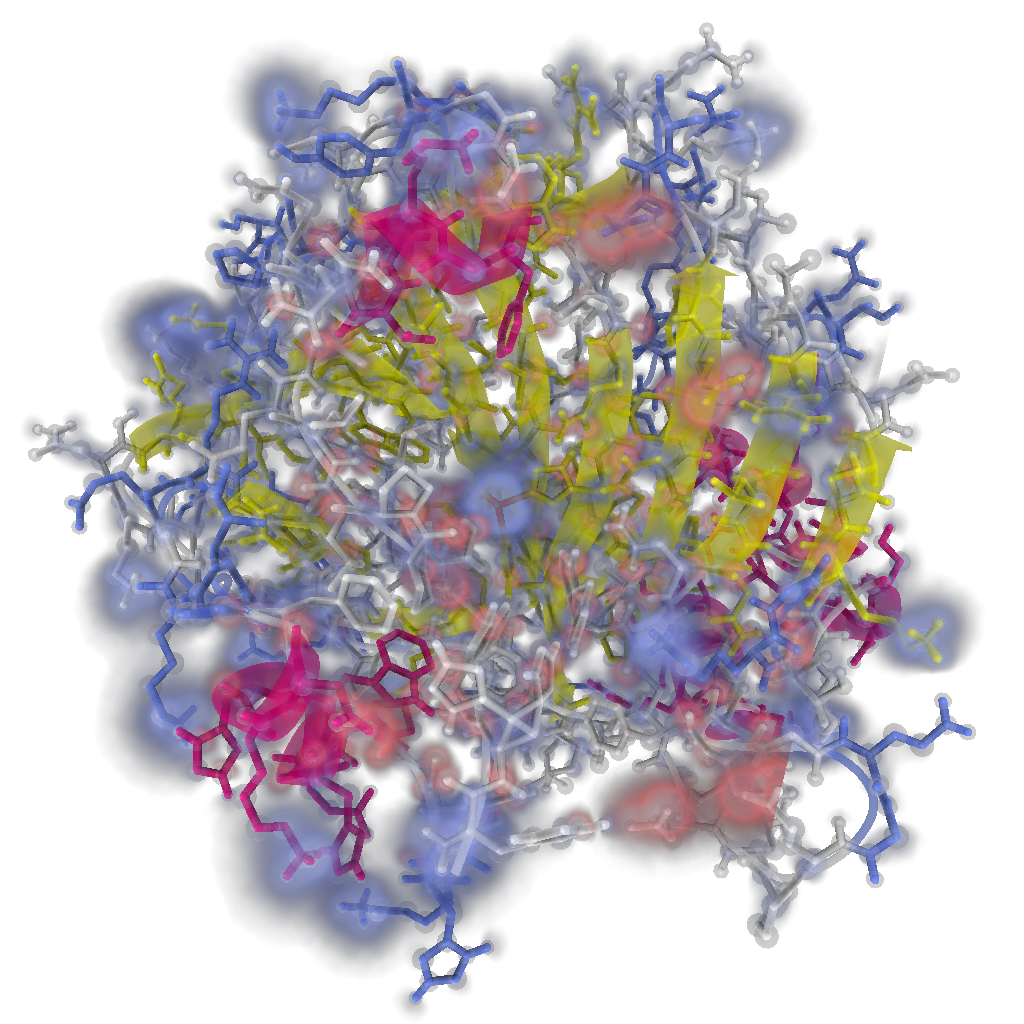
\includegraphics[width=\linewidth]{snapshots/mol/cgf/render}%
      \subcaption{\label{fig:sub:protein}%
        hybrid visualization
      }%
    \end{minipage}%
  }
  \settoheight{\boxheight}{\usebox\savedProteinBox}
  % 
  \begin{minipage}[b][\boxheight][b]{0.24\linewidth}
    \centering%
    \begin{minipage}[t]{0.98\linewidth}
      \centering
      \setlength{\imgWidth}{\textwidth}
      \splitImage{snapshots/mol/cgf/g1}{snapshots/mol/cgf/g2}\vspace{-4mm}
      \subcaption{\label{fig:sub:protein-geoms}%
        geometric data
      }
    \end{minipage}%
    \vfill%
    \begin{minipage}[b]{0.98\linewidth}
      \centering
      % 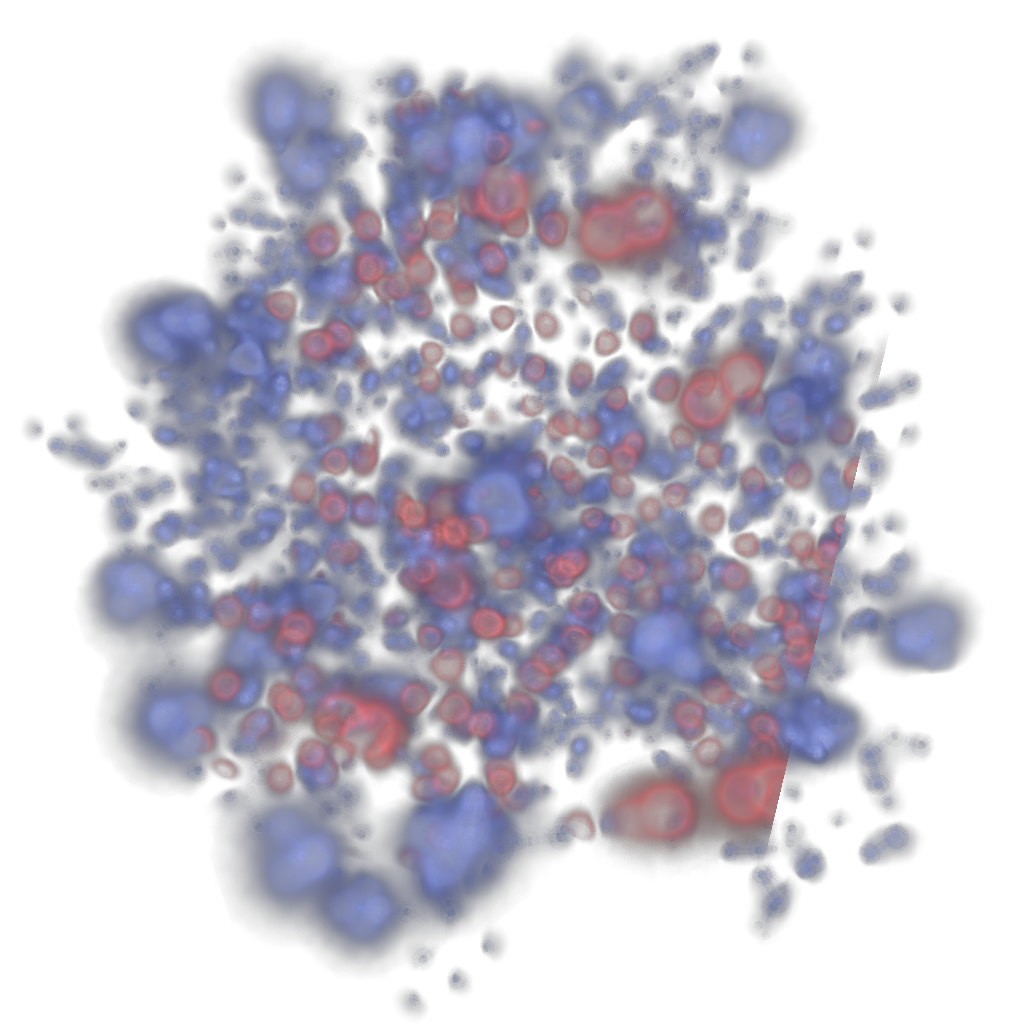
\includegraphics[width=0.98\linewidth]{snapshots/mol/cgf/vols}
      \setlength{\imgWidth}{\textwidth}
      \splitImage{snapshots/mol/cgf/v1}{snapshots/mol/cgf/v2}\vspace{-4mm}
      \subcaption{\label{fig:sub:protein-vols}%
        volume data
      }
    \end{minipage}%
  \end{minipage}%
  \hfill%
  %% central image
  \usebox\savedProteinBox
  \hfill%
  \begin{minipage}[b][\boxheight][b]{0.24\linewidth}
    \centering%
    \begin{minipage}[t]{0.98\linewidth}
      \centering
      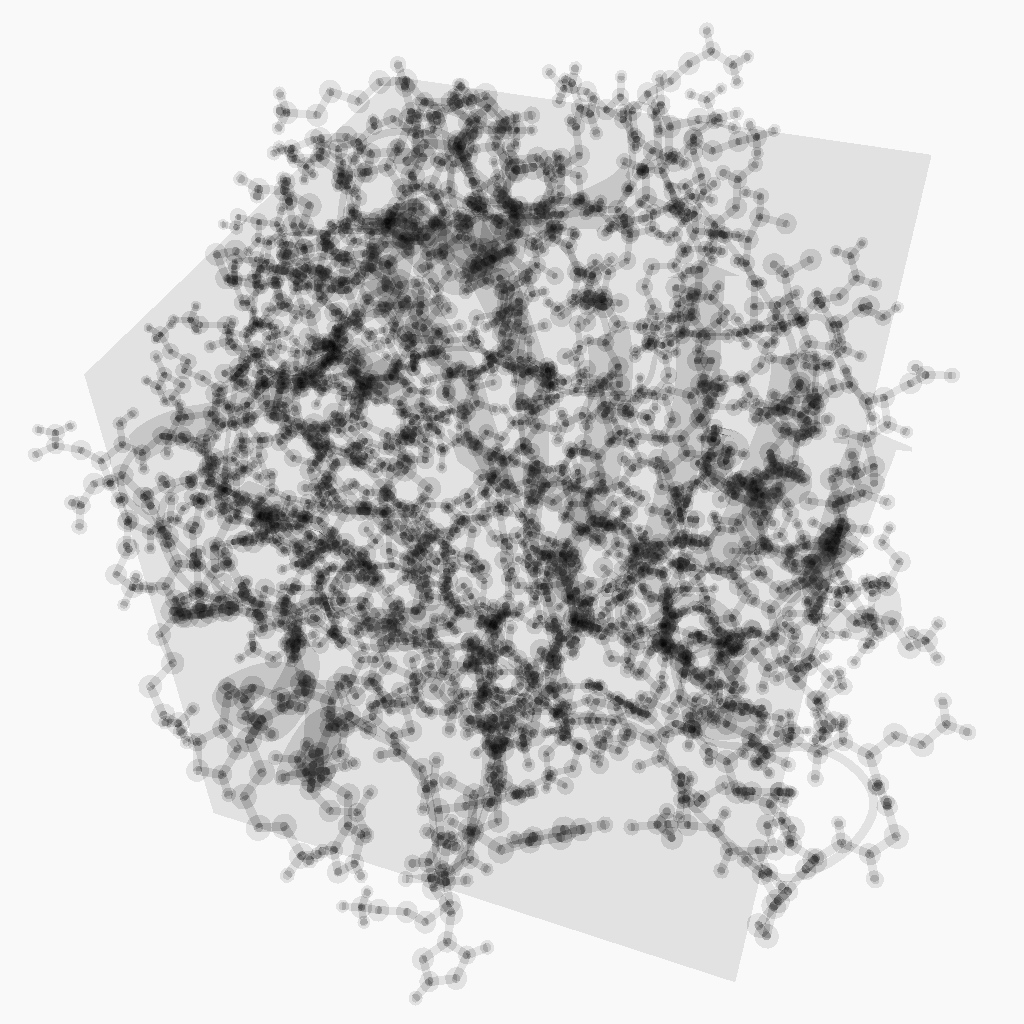
\includegraphics[width=\linewidth]{snapshots/mol/cgf/dci-scaled-inv}
      \subcaption{\label{fig:sub:protein-dci}%
        depth complexity
      }
    \end{minipage}%
    \vfill%
    \begin{minipage}[b]{0.98\linewidth}
      \centering
     %\includegraphics[width=\linewidth]{snapshots/mol/cgf/dch-64-max46}
      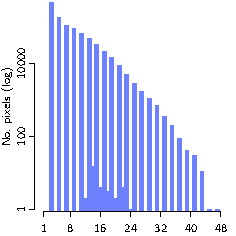
\includegraphics[width=1\linewidth]{figures/plot-dch-mol}\vspace{-2mm}
      \subcaption{\label{fig:sub:protein-dch}%
        depth complexity histogram
      }
    \end{minipage}%
  \end{minipage}%
  % 
  \caption{\label{fig:protein}%
    Visualization of a protein (PDB-ID: 2CBA) combining hybrid data from different sources.
    (\subref{fig:sub:protein}) final rendering of hybrid visualization.
    (\subref{fig:sub:protein-geoms}) geometric protein representations. 
    (\subref{fig:sub:protein-vols}) volumetric data sources depicting electrostatic potentials. 
    (\subref{fig:sub:protein-dci}) image-space depth complexity (re-scaled for representational purposes). 
    (\subref{fig:sub:protein-dch}) depth complexity histogram (DCH, log scale). %% showing a maximum of $46$ depth layers. 
    Our improved, \ab{}-based rendering algorithm is capable of rendering the entire scene at 32\,fps---a performance increase of $5.9$ times relative to prevalent techniques. %perfnumber
    %Such protein visualizations are commonly used molecular sciences to investigate possible docking sites. 
  }
\end{figure*}



\section{Visualization of Scenes with Non-uniform Depth Complexity}
\label{sec:depthcomplexity}

In this paper, we have chosen four representative scenes of different fields including molecular science, medical treatment planning, space weather simulations, and computational fluid dynamics. A major computational cost, characteristic for the selected scenes, arises from the task of ordering all contributions in terms of visibility. In modern OIT solutions, these costs are directly related to the observed depth complexity in the image.
That is, the number of overlapping contributions per pixel. 
%
At the same time, most natural scenes often feature non-uniform complexity distributions in image space with clusters of high complexity surrounded by regions of lower complexity. To analyze the complexity of such scenes we use depth complexity histograms.


\subsection{Depth Complexity Histograms}
\label{sec:dch}
   
We use the term Depth Complexity Histogram (\dch) for a histogram that plots the distribution of depth complexities for all pixels given a specific scene and camera setting. 
Each bin in a \dch\ is associated with a complexity range and holds the number of pixels whose depth complexities fall within that range (cf.\ Figure~\ref{fig:protein}(\subref{fig:sub:protein-dch})). 
Computing a \dch\ can be done by first rendering an integer image of the scene where each pixel holds the number of contributing fragments and the pixel value is treated as an atomic counter. The \dch\ can then be computed as a standard histogram over this integer image.


\begin{figure}[t]
  \centering
  \begin{minipage}{1.0\linewidth}\centering
    \fbox{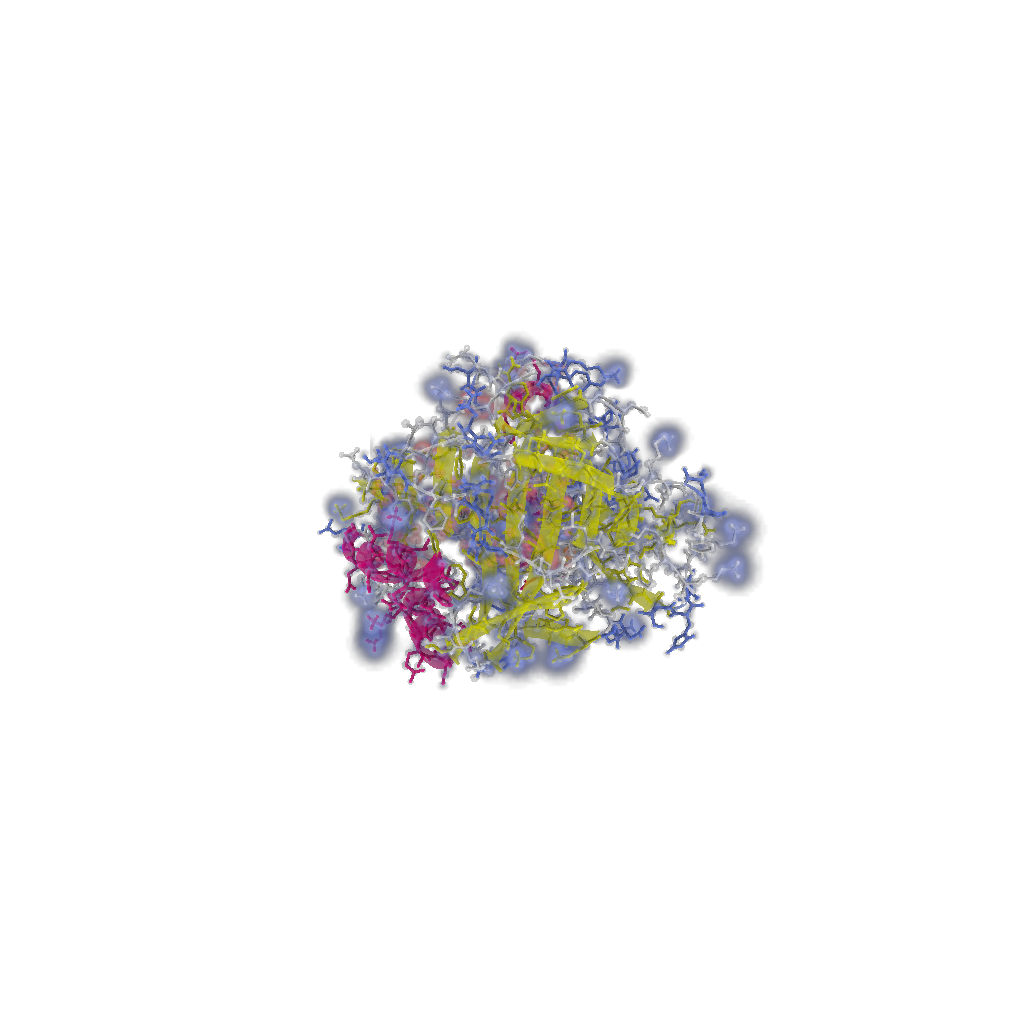
\includegraphics[width=0.16\linewidth]{snapshots/mol/cgf/viewdep/0050}}%
    \hfill%
    \fbox{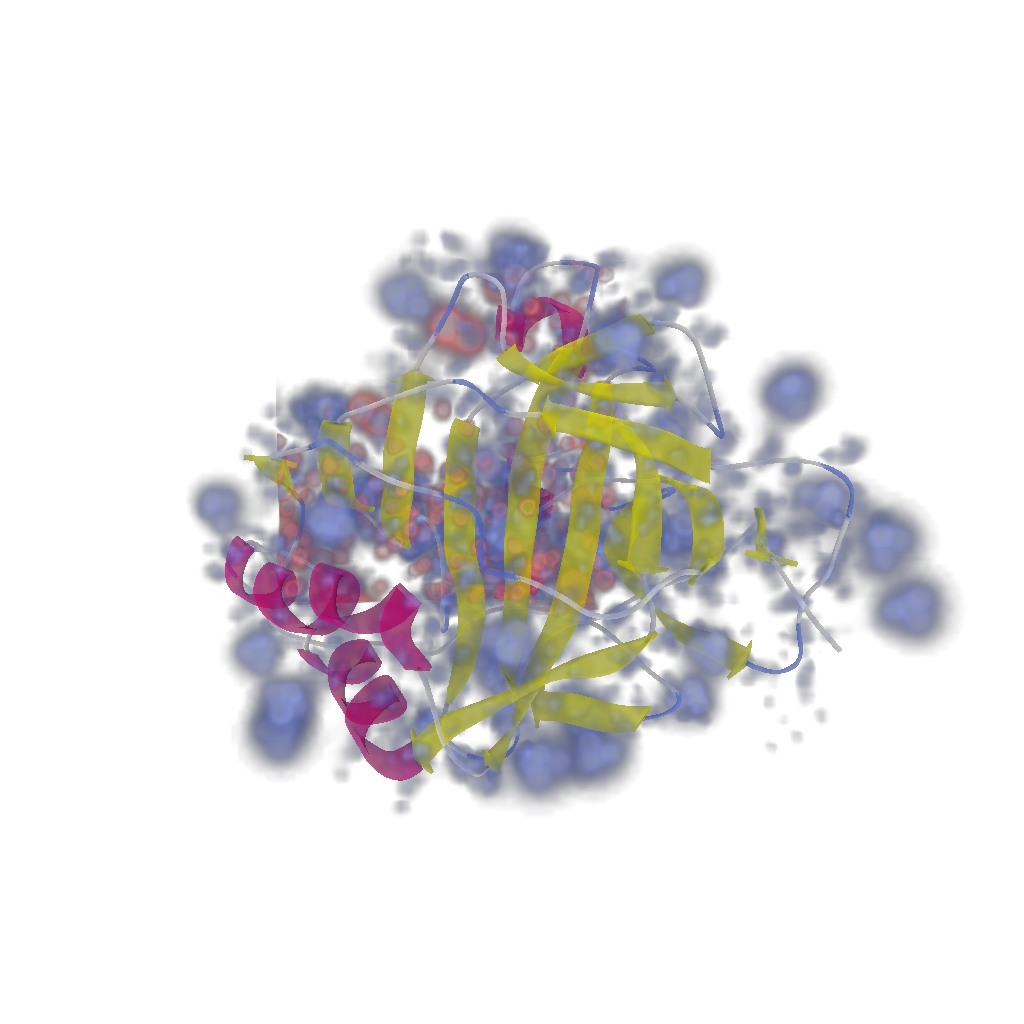
\includegraphics[width=0.16\linewidth]{snapshots/mol/cgf/viewdep/0150}}%
    \hfill%
    \fbox{\includegraphics[width=0.16\linewidth]{snapshots/mol/cgf/viewdep/0250}}%
    \hfill%
    \fbox{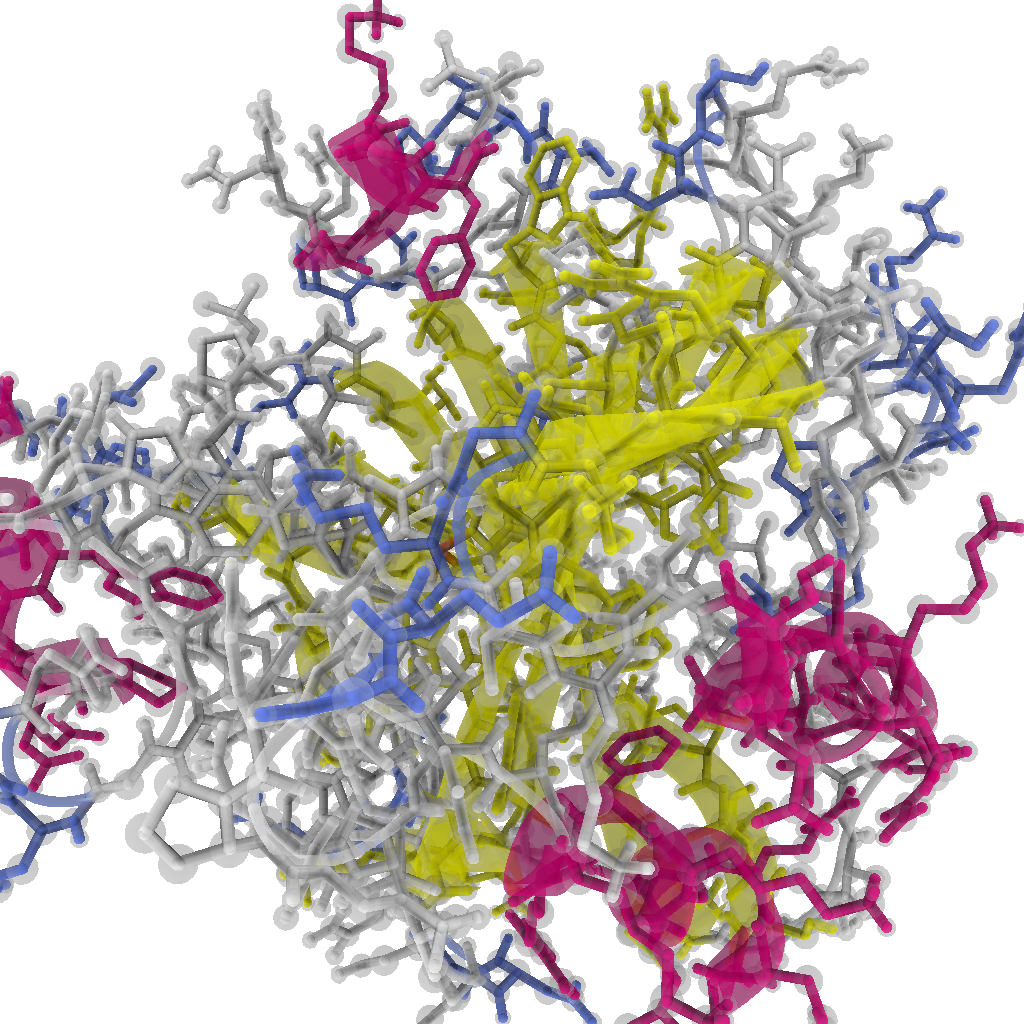
\includegraphics[width=0.16\linewidth]{snapshots/mol/cgf/viewdep/0350}}%
    \hfill%
    \fbox{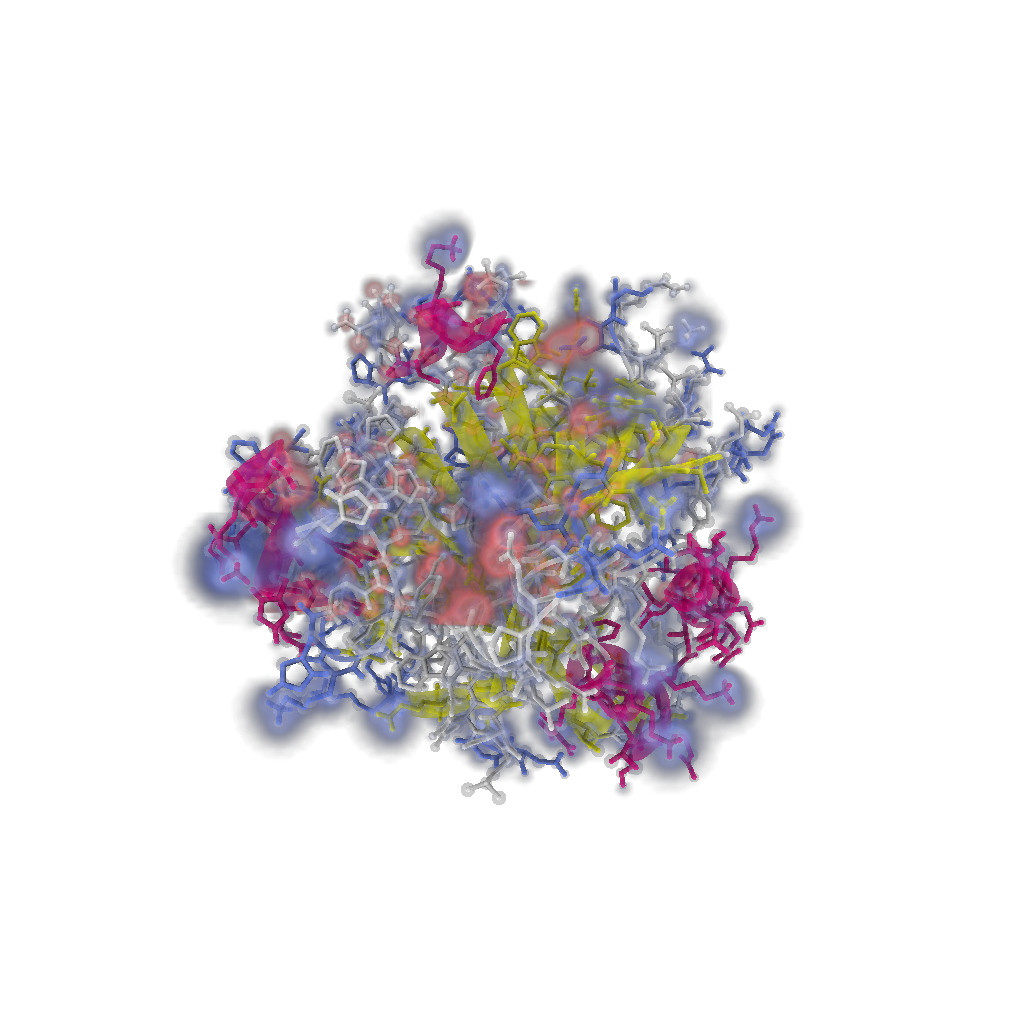
\includegraphics[width=0.16\linewidth]{snapshots/mol/cgf/viewdep/0450}}%
    \hspace{9mm}
  \end{minipage}\\
  % 
  \begin{minipage}{1.0\linewidth}\centering
    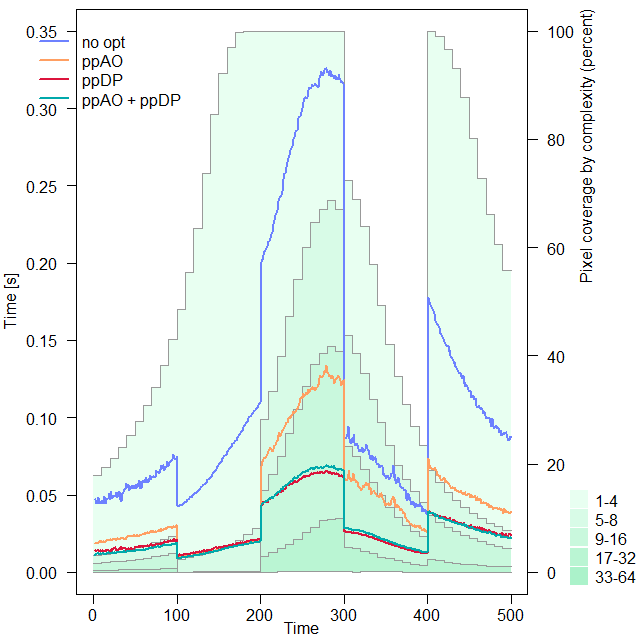
\includegraphics[width=\linewidth]{figures/placeholder_viewdep} 
  \end{minipage}
  % 
  \caption{\label{fig:viewdep}%
    Performance and complexity graphs as a function of time for a predefined camera path around the protein data set from Figure~\ref{fig:protein}. 
    The plot shows rendering times (lines, left y-axis) and \dch{}s (bar charts, right y-axis). 
    The camera path goes \emph{far}$\rightarrow$\emph{near}$\rightarrow$\emph{far} and the sequence contains abrupt changes in scene composition at every $100\textsuperscript{th}$ time-point. 
    At the first marker (orange), the geometry of the stick representation is removed (cf.~Figure~\ref{fig:protein}(\subref{fig:sub:protein-geoms})) reducing high-complexity pixels. 
    At the second marker (green), both volume data sources are removed (cf.~Figure~\ref{fig:protein}(\subref{fig:sub:protein-vols})) reducing low-complexity pixels. 
    The top row corresponds to snapshots from the different sections of the sequence. 
  }
\end{figure}



\subsection{Visualization Challenges for Data Fusion}
\label{sec:vischallenges}

During the analysis of our four scenes, we made the observation that many pixels feature a low depth complexity and only a few pixels feature the highest depth complexities. 
This results in rapidly decreasing \dchs\ where the majority of pixels have a complexity that is only a fraction of the global maximum of the scene.
In our opinion, these findings can also be generalized to other scenes.

% Molecular
%
One example, the protein \emph{human carbonic anhydrase II}, is depicted in Figure~\ref{fig:protein}. 
The scene consists of two polygonal representations of protein structures and two volumetric sources containing the electron charge density. 
Such protein visualizations are commonly used to examine possible docking positions between the protein and other molecules~\cite{Seeliger2010}. 

From a depth complexity perspective, the protein scene is relatively well behaved.
The maximum depth complexity is not particularly high and the points with high depth complexity are evenly distributed across the entire scene. 
However, as can be seen in Figure~\ref{fig:protein}(\subref{fig:sub:protein-dch}), the \dch{} decreases rapidly. 
The majority of all pixels ($68\,\%$) have a depth complexity of 8 or less, whereas only very few ($6.6\,\%$) have a complexity higher than 17 with a maximum of 46 for the particular camera setting. 
%Similar trends are also found in scenes with more pronounced focus-context character, such as the fiber-tracts of the neurosurgery scene (Figure~\ref{fig:neuro-flow}(\subref{fig:sub:neuro})) or the streamlines of the flow scene (Figure~\ref{fig:neuro-flow}(\subref{fig:sub:flow})), both of which have considerably higher maximum complexity than the Protein scene. 


The \dch{} for a particular scene is naturally view-dependent. 
Figure~\ref{fig:viewdep} provides an analysis of how the \dch{} changes for the protein scene during a scripted sequence. 
(The \dch{} for each time step is plotted vertically as a stacked bar chart of relative screen coverage in percentages.) 
In addition to camera movement, the sequence also contains changes in the scene construction at every $100\textsuperscript{th}$ time-point, such as removal of geometry at $t=100$ (re-added at $t=200$) and removal of both volumes at $t=300$ (re-added at $t=400$). 
Even with the camera very close to the protein the \dch{}s shows that the complexity is still non-uniform, opening up the possibility for significant savings if dynamic memory management can be used to avoid redundant array sizes. 
%The next section provides a technical description of why current state-of-the-art OIT techniques are only \emph{partially} able to adapt to non-uniform scene complexity. 
Next, we provide a technical description of how current state-of-the-art OIT techniques adapt to such non-uniform scene complexity. 


\newcommand{\bFraglist}{Fragment List}

\newcommand{\bTarget}{Render Target}
\newcommand{\bAnchor}{List Anchor}
\newcommand{\bPool}{Fragment Pool}
\newcommand{\bAtomic}{Atomic}
\newcommand{\bSemaphore}{Semaphore}
\newcommand{\bArray}{Local Array}
\newcommand{\bCounter}{Complexity Counter}

\newcommand{\sClear}{Clear Step}
\newcommand{\sFill}{Fill Step}
\newcommand{\sResolve}{Resolve Step}

\newcommand{\sCount}{Count Step}
\newcommand{\sSegment}{Segmentation Step}
\newcommand{\sTrigger}{Per-Segment Resolve}

\newcommand{\las}{L} %Local Array Size
\newcommand{\abs}{ABuffer\_s}







\begin{figure}[t]
  \centering
    %\def\svgwidth{\linewidth}%
    \graphicspath{{figures/}}%
    %% change font within next curly braces, e.g. \sffamily\footnotesize
    {\sffamily\footnotesize\input{figures/abuffer-flowchart.pdf_tex}}
    %
  \caption{\label{fig:abuffer-flowchart} 
	Overview of the \ab{} rendering loop as implemented on GPU hardware. 
	Previous literature has focused primarily on the global memory management during the \sFill. 
	Our proposed algorithm additionally improves the management of local GPU cache memory. 
	Memory related steps are highlighted in blue.
   }
\end{figure}


\section{Algorithms for Semi-Transparent Data Fusion}
\label{sec:oit-global}

To construct an algorithm optimized for scenes with non-uniform depth complexity, we exploit the knowledge gained from analyzing depth complexities as described in the previous section. 
Three state-of-the-art implementations of the well-known \ab{} concept serve as a reference.
We direct the interested reader to the survey provided by Maule \etal~\cite{Maule2011} for a comprehensive introduction to raster-based transparency techniques.
This section details the differences of the algorithms in the dynamic management of \emph{global} GPU memory.
In addition, we show how to further optimize the algorithms with respect to their use of \emph{local} caches on modern graphics hardware.

\begin{figure*}[t]
  \centering
    \def\svgwidth{\textwidth}%
    \graphicspath{{figures/}}%
    %% change font within next curly braces, e.g. \sffamily\footnotesize
    {\sffamily\footnotesize\input{figures/algorithm-overview.pdf_tex}}
    %
  \caption{\label{fig:abuffer-global} 
    Comparison of three existing \ab{} implementations for managing global GPU memory. Both the DFB and PPLL approaches adapts well to scenes with non-uniform depth complexities and decreasing \dchs\ by allowing dynamic memory usage. 
  }
\end{figure*}


%\subsection{Dynamically Sized \ab{}s on Modern GPUs}
%\label{sec:ab-merged}
%\todo{no subsection if there is no 4.2! /M}

The principle of the \ab{} is to capture and store a list of rasterized fragments on a per-pixel basis (called \emph{\bFraglist}). 
As illustrated in Figure~\ref{fig:abuffer-flowchart}, this involves three sequential steps: the \sClear, the \sFill, and the \sResolve. 
Both the \sFill{} and \sResolve{} contain sub-steps associated with memory management (highlighted in blue). 
This includes global memory management mainly during the \sFill and local cache management in the \sResolve.
The particular data structure of fragments and further considerations on source types will be described in Section~\ref{sec:fusion}.





\subsubsection*{Managing Global GPU Memory}

Three prevalent approaches for managing the global \ab{} memory during the \sFill{} are used.
These are Fixed Fragment Buffers~\cite{Crassin2010}, Dynamic Fragment Buffers~\cite{Maule2012}, and Per-Pixel Linked Lists~\cite{kainz2009ray,Yang2010,Crassin2010} (FFB, DFB, and PPLL, respectively). 

The FFB, DFB, and PPLL approaches are all illustrated side-by-side in Figure~\ref{fig:abuffer-global}.  
Each pixel is associated with a fragment counter and an implicit or explicit pointer to the beginning of the stored \bFraglist. 
For the FFB the global memory pool is statically partitioned and the pointer is implicitly given by the screen coordinates of the fragments. 
The global memory pool of the DFB is dynamically partitioned each frame and the explicit pointer holds a base offset into the pool. 
For the PPLL the pointer denotes the list anchor for a linked list of fragments spread throughout the pool. 
Both, FFB and DFB ensure a contiguous memory layout for each individual pixel. 
The \bFraglist s are generally stored out-of-order (unsorted) in the relatively slow but large global memory of the GPU.

DFB and PPLL are dynamic algorithms and adapt the utilization of global memory well to non-uniform depth complexity distributions. 
As a result, consumption of global memory is almost optimal even for rapidly decreasing \dch{}s. 


\begin{figure*}[t]
  \centering
  \def\svgwidth{\textwidth}%
  \graphicspath{{figures/}}%
  %% change font within next curly braces, e.g. \sffamily\footnotesize
  {\sffamily\footnotesize\input{figures/algorithm-optimization.pdf_tex}}
  % 
  \caption{\label{fig:abuffer-local} %
    Comparison of approaches for managing local GPU caches; showing static management (the dominant approach in the literature) and our two optimizations: \stencil{} and \dloop{}.
    The (unsorted) input \bFraglist{} (top) corresponds to the output of the \sFill{} and resides in global memory (cf.\ FFB, DFB or, PPLL in Figure~\ref{fig:abuffer-global}). 
    The array is sorted  in local caches during the \sResolve{} using predefined array sizes. 
    Two pixels are exemplified, a heavy pixel (blue) and a light pixel (orange). 
    The \stencil{} optimization significantly lowers the amount of unused memory (shown in gray), while the \dloop{} optimization lowers both the unused as well as the used memory (though re-usage). 
    \stencil{} and \dloop{} can be used together or separately.
  }
\end{figure*}


\subsubsection*{Managing Local GPU Caches}

It is common practice to copy the (unsorted) \bFraglist\ from global memory to local cache before sorting, thereby avoiding the relatively high latency of the global memory during the read/write intensive sorting procedure. 
An important aspect of cache usage is that the memory layout of modern GPUs typically expose a limited shared cache to a group of cores. 
Additionally, modern GPUs are capable of hiding global memory latency by 'hot swapping' groups of threads in a manner similar to pipelining on a CPU~\cite{Nvidia2011}. 
Under ideal circumstances, the number of active threads can be up to eight times the number of physical cores. 
For this to be possible, the allocation per thread needs to be small enough, such that all active threads designated to a group of cores can have their arrays allocated simultaneously. 
It is therefore important to minimize the allocation of cache memory to maximize performance. 
The current trend is also that the number of cores increase faster than the available shared cache size, potentially escalating this problem in the future. 

The dominant approach described in the literature for managing local GPU caches is to allocate a fixed sized array, of size $N$, per thread. 
This has two immediate consequences. 
First, the maximum depth complexity of the system is limited to $N$, as all fragments beyond this number are discarded (the memory is only used once per thread). 
Second, larger array sizes significantly reduce the number of active threads (due to cache overflow and reduced 'hot swapping'). 
A number often reported in the literature is $N=64$. 
Hence, while the literature includes strategies, such as DFB and PPLL, for managing the global memory, there remains room for improvement in the management of local caches.


\section{Improved Dynamic Depth Complexity Management}
\label{sec:oit-local}

We propose two optimizations for the \ab{} algorithm based on the observed nature of the \dchs{} described earlier. 
Both optimizations are designed to improve the management of local GPU caches. 
For clarity, we will use the term \bArray{} to indicate the fast memory allocated for the sorting of fragments. 

The first optimization, illustrated in the center of Figure~\ref{fig:abuffer-local}, ensures that all pixels are evaluated without allocating excessively large \bArray{}s. 
To achieve that, the image space is segmented into sections of similar depth complexity and separate shaders, compiled with different local arrays sizes, are triggered for each segment. 
The optimization is hence denoted \emph{per-pixel Array Optimization} (\stencil). 
The second approach (Figure~\ref{fig:abuffer-local}, right), is part of the \sResolve\ and corresponds to a novel sorting procedure, called per-pixel Depth Peeling (\dloop) that breaks sorting into smaller pieces by not loading all fragments at once. 
The approach shares similarities to depth peeling as it iteratively sorts and resolves part of the entire list, but does so fully on the GPU between global and local memory without need to re-render geometry. 

An important aspect of both \stencil{} and \dloop{} is that they are designed to be used \emph{together} with the current state-of-the-art management of global memory described in the previous section. 
Our full rendering algorithm, optimized for geometry intensive fusion scenes, is thus created by combining existing solutions, such as DFB or PPLL, with the approaches presented here. 


\subsection{Dynamic Resource Management Using Per-pixel Array Optimization (\stencil)}
\label{sec:ppao}

The objective of the proposed per-pixel Array Optimization (\stencil{}) is to limit the amount of unused memory in the local cache by performing the \sResolve{} with \bArray{}s that better correspond to the depth complexity of individual pixels. 
Since dynamic memory allocations are not possible at the highest cache levels of the GPU memory hierarchy, the optimization of per-pixel array sizes requires multiple shader programs to be instantiated with varying \bArray{} sizes.
Rather than using a unique shader for every possible \bArray{} size we use a smaller set of pre-defined array sizes. 
This leads to a binning of the \dch{}, i.e.\ clustering of pixels with similar depth complexity into complexity segments. 
All pixels in a complexity segment are then resolved as a batch by a single shader. 
The full image is then processed in as many batches as there are complexity segments. 
Note that the clustering does not depend on the location of the pixels and that each segment therefore not necessarily corresponds to a focused region in the image. 
The \stencil{} is positioned after the \sFill{} in the \ab{} algorithm (cf.~Figure~\ref{fig:abuffer-flowchart}) and make the \stencil{} responsible for managing and calling the \sResolve{} on the respective complexity segments.

%Since dynamic memory allocations are not possible at the highest cache levels of the GPU memory hierarchy, the optimization of per-pixel array sizes requires multiple shader programs to be instantiated with varying \bArray{} sizes.
%This allows for dealing with different classes of complexity segments. 
The instantiation procedure of the shader programs is straightforward as the individual instances only differ by a single number; the predetermined buffer size. 
It is also sufficient to instantiate only a small set of shaders due to the decreasing power curve observed in most \dch{}s. 
By analyzing the depth complexity of various scenes, we found that complexity segments of sizes 8, 16, 32, and and so on give good results with respect to performance and memory consumption.

The \stencil{} algorithm is outlined below.
%
%% begingroup/endgroup stuff is necessary for placing the algorithm exactly here ([H]) in two-column mode
\begingroup
\removelatexerror% Nullify \@latex@error
\begin{algorithm}[H]
  %
  %$C \longleftarrow {8, 32, 128}$\; // set of complexity segments
  % count depth complexity $\forall$ pixels during \sFill\;
  \tcp{\sFill}
  \ForAll{pixels of the framebuffer}{ 
    count depth complexity;
  }
  \tcp{\sResolve, loop over all complexity segments}
  \ForEach{$i \in \{8, 16, \dots, \mathrm{max}\}$}{
    activate shader program for complexity segment $i$\;
    \ForEach{pixel $p \in$ pixels}{
      \tcp{mask pixels if not part of segment class $i$}
      \If{$\mathrm{depth\ complexity}(p) = i$}{
        resolve segment with \bArray{} of size $i$\;
      }
    }
  }
\end{algorithm}
\endgroup

To perform \stencil, we need to know the depth complexities of all pixels. 
For this purpose, we utilize an integer buffer the size of the framebuffer to count the number of fragments per pixel.
The counting can be performed during scene rasterization (the \sFill{}) and thus no additional rendering passes are required.

Once the depth complexities are known, the different complexity segments may be processed. 
This is done by looping over all pre-defined sizes of complexity segments and activating the shader program with the respective \bArray{} size. 
The clustering of pixels into complexity is handled implicitly during runtime by a masking step where all all pixels that are not part of the current segment are discarded. 
%Pixels whose depth complexity is part of the current complexity segment are resolved. 
%All other pixels are discarded. 
Note that the graphics pipeline does not need to be flushed between triggering successive segments and that multiple segments may be evaluated in parallel (even if they are triggered sequentially). 
Figure~\ref{fig:abuffer-local}, center, depicts the utilization of our approach for pixels exhibiting high and low depth complexity.


\subsection{Preventing Over-sized Local Arrays Using Per-pixel Depth Peeling (\dloop)}
\label{sec:ppdp}

If the number of fragments inside a \bFraglist{} exceeds the buffer size of the \bArray{}, usually information is lost and the final rendering result might feature artifacts.
One impractical solution is to increase the size of the \bArray{}s, but since typically only a few pixels exhibit a high depth complexity (cf.~Section~\ref{sec:dch}) large parts of the pre-allocated memory will never be used (cf.~Figure~\ref{fig:abuffer-local}, left).
To overcome this particular problem, we propose a variation of depth peeling on a per-pixel level to provide a simple way to correctly deal with overflowing \bArray{}s.
Thus, the maximum supported depth complexity is no longer limited by the size of local memory but instead restricted only by the available global memory.
In Figure~\ref{fig:abuffer-local}, right, a \bArray{} size of 8 is used to illustrate our approach for two different depth complexities.

The \dloop{} algorithm is outlined below and replaces the \sResolve{} for individual pixels in Figure~\ref{fig:abuffer-flowchart}.
%
%% begingroup/endgroup stuff is necessary for placing the algorithm exactly here ([H]) in two-column mode
\begingroup 
\removelatexerror% Nullify \@latex@error
\begin{algorithm}[H]
  \def\FragList{fragment list}
  \def\Buffer{buffer} %% local Cache
  \def\MinDepth{min depth}

  \def\State{current state}
  \def\Depth{depth}
  \SetKwInOut{Input}{input}
  \SetKwInOut{Output}{output}
  %
  \Input{list of fragment data per pixel} 

  $n \leftarrow $ sizeof(\bArray{})\;
  create \Buffer{} with $n$ elements\;
  set \MinDepth{} to 0\;
  initialize \State\;
  
  \Repeat{all fragments $f \in $ \FragList{} are resolved}{%
    \ForEach{fragment $f \in $ \FragList{}}{
      \eIf{\Depth($f$) $\ge$ \MinDepth}{
        discard $f$ in current pass\;
      }{
        insert $f$ into \Buffer{} enforcing sorting\;
        \tcp{store at most $n$ elements}
      }
    }
    resolve \Buffer{} considering \State\;
    store \MinDepth{} and state of last \Buffer{} element\;
%    store \State{} of last \Buffer{} element\;
    clear \Buffer\;
  }
\end{algorithm}
\endgroup

The principal idea follows the approach of bucket depth peeling where a larger list is sorted and resolved as a set of smaller sequences. 
Here, we split the \sResolve{} into several subpasses which allows for the \bArray{} to be re-used and its size to be reduced. 
With a \bArray{} of size $n$, the process sorts $n-1$ elements in the \bFraglist{} per subpass. 
Sorting the full array thus takes a maximum of $D/(n-1)$ passes (rounded up), but may be terminated sooner, such as in the case of early ray termination. 
In case the process is interrupted, remaining passes are skipped and further read/write intensive sorting operations are avoided. 
Note that the size of the \bArray{} remains predefined and, thus, constant. 
Observed optimal \bArray{} size for \dloop{} purposes was $8$ across all our test setups with respect to performance. 

While looping over the contents of the \bFraglist{}, the $n$ entries with the smallest depth values are chosen and stored in sorted order in the buffer by using insertion sort.
If a fragment was already processed in an earlier pass, its depth will be smaller than the current minimal depth and it is thus discarded for the current pass.
After the buffer is filled up, the buffer contents are resolved. 
With a \bArray{} size of $8$, fragments $0$--$8$ would be sorted in pass $1$, fragments $9$--$16$ in pass $2$, etc. 
To ensure consistency between the individual resolve passes, we consider the current state of the rendering including volumetric flags or other meta data.
Afterward, the current state and minimal depth are updated and the local buffer is emptied for the next pass. 
The process does not require additional rendering passes but does require the entire \bFraglist{} to be read multiple times from global GPU memory. 

Note that the \dloop{} algorithm may exhibit z-fighting issues similar to regular depth peeling. 
The issue arises when multiple fragments of a single pixel have identical depth values and only a subset of these fragments gets included in a loop iteration. 
Since only the minimal depth is used to distinguish processed fragments from fragments yet to be resolved, the solution is not unique.
This also complicates the decision in the following iterations regarding which fragments should be discarded.
However, this phenomenon of multiple identical depth values inside the data is rather rare and we have so far not experienced any artifacts from this form of z-fighting. 
A potential way to handle the problem is to introduce an additional flag per fragment entry whether it has been resolved.
But that will also include an additional test increasing the computational load thereby.


\section{Fused Rendering of Hybrid Data Sources}
\label{sec:fusion}

The outline of the \ab{} rendering loop is illustrated in the flowchart in Figure~\ref{fig:abuffer-flowchart}. 
So far we have focused mostly on the memory management involved in the construction of the sorted \bFraglist{} (steps highlighted in blue). 
In this section, we will focus on its evaluation and the rendering of the scene (orange highlight) as well as the use of specific data structures . 

\newcommand{\ccz}{\emph{z}}
\newcommand{\ccid}{\emph{id}}
\newcommand{\cccol}{\emph{col}}

\subsection{\bFraglist\ Creation and Evaluation}

The following data structure is used for all fragments produced in the \sFill\ as entries of the \bFraglist:
\begin{description}[font=\normalfont\itshape]
\item[\abs:] \emph{float32 z}, \emph{int32 id}, \emph{vec4 float16 col}.
\end{description}
The structure has a total size of 16 bytes and the same data structure is used for both geometric and volumetric contributions. 

During the \sFill, \abs\ entries are computed and stored in the \bFraglist. 
Geometric sources are shaded during this step and the computed color is stored explicitly in the \cccol\ component. 
For volumetric sources, only the associated proxy geometry is rendered during the \sFill\ and the \cccol\ component is left uninitialized. 
The \ccz\ and \ccid\ components are treated identically for all source types and respectively hold the depth value in screen space coordinates and a unique source identifier. 
Bit operations are used on the \ccid\ component to store both source type as well as a unique identifier. 
Sources may be rendered independently by different shaders but the produced fragments (instances of \abs) are all inserted into the same global storage.

During the final stage of the \sResolve, the scene content is evaluated and blended into the framebuffer. 
At this point, all entries in the \bFraglist\ can be interpreted as intersection points along the view direction. 
The spatial position of these intersections are computed as (un-)projections of the depth value from screen to world coordinates. 
Ray casting of the scene is thus executed in world space by sequentially looping over all entries in the \bFraglist. 
As they are encountered, geometry fragments are blended directly to the buffer while volume rendering is performed on the intervening ray segments. 
Volume occupancy is tracked through a bitmask integer which is updated every time a fragment from a volume proxy geometry is encountered. 
For more information on \bFraglist\ evaluation, particularly the use of bitmasks to track volume occupancy, we direct the reader to~\cite{brecheisen08multimodal}. 
Entry and exit points for a local ray segment is available in world coordinates from the enclosing fragments' \ccz\ components. 
Once the occupancy and entry/exit points are known, the problem is reduced to the problem of multi-volume rendering as described in the literature on multi-volume fusion. 


\subsection{Implementation Details}

%As previously stated, the methods presented in this paper are compatible with most current work that optimizes \ab{} memory management on a global level. 
Our implementation supports global memory management using FFB, DFB and PPLL as described in Section~\ref{sec:oit-global}. The FFB and PPLL implementation used in our implementation are derived from~\cite{Crassin2010} (freely available) while the DFB implementation is derived from~\cite{Maule2012} (proprietary). Implementation was done in C++, OpenGL and GLSL with the only exception being the `scan' step in the DFB implementation which is performed in CUDA (using Thrust) as explained in~\cite{Maule2012}. 
%Unfortunately, this forced an expensive context switch on all our setups, causing a $50$--$200$ ms rendering penalty depending on the hardware. The impact of this penalty will be discussed further in Section~\ref{sec:results}. 

For management of local cache memory we use the \stencil\ and \dloop\ as presented in Section~\ref{sec:oit-local}. 
The \stencil\ optimization is currently implemented using an 8bit stencil buffer in order to select which parts of the image that should be triggered by a particular shader. 
The \sFill\ is thus enclosed in a loop at the C++ level where different segments are triggered by varying the OpenGL stencil function. 
Note that using an $8$bit buffer in this manner does not limit the depth complexity to $255$ (higher complexities are still possible but will all be triggered as the same segment). 
If higher segment limits are needed, the stencil buffer can easily be replaced with a higher precision integer texture. 
The \dloop\ optimization simply replaces the final steps of the \sResolve\ and is implemented as a loop directly in GLSL. 

The \bArray{}s are always allocated as local arrays with predefined sizes inside the shaders and are thus not assigned explicitly to any specific memory. 
Thread scheduling and memory assignment is therefore up to the discretion of the driver and thus not necessary to perform manually. 

The full algorithm, with global and local optimizations, requires the implementation of three shaders (clear, fill, resolve), plus additional clones of the resolve shader for \stencil\ purposes.




\section{Results}
\label{sec:results}

%\todo{Reviewer 5: I would like to see images for each one of the separated datasets that compose one scene.}

The presented algorithm have been tested on four real-world cases from different fields:
\begin{description}[font=\normalfont\itshape]
\item[Figure~\ref{fig:protein}, Protein:]% 
%The data corresponds to the protein 2CBA. The scene consists of four separate data sources; two volumetric data sets describing the electron charge density at different resolutions and extent, a geometric ``stick'' representation of the protein, and a geometric ``ribbon'' model of the protein, both colored by secondary structure identity. The three-dimensional structure and charges are frequently used to examine possible docking positions between the protein and secondary materials~\cite{Seeliger2010}.
The data corresponds to the protein `human carbonic anhydrase II'. The scene consists of four separate data sources; two volumetric data sets describing the electrostatic potential calculated at different resolutions and extent, a geometric stick representation of the protein, and a geometric ribbon model of the protein, both colored by secondary structure type. The three-dimensional structure and potential fields are often visualized to examine possible docking positions between the protein and other molecules~\cite{Seeliger2010}.
\item[Figure~\ref{fig:space}, Space:]% 
This data set depicts a multi-variate simulation of a time-dependent 3D MHD simulation of the heliosphere during a coronal mass ejection event as it is currently used in space weather prediction~\cite{Xie2004}. The scene consists of two volumes, showing the number of charged particles and the energy density respectively, and three iso-surfaces derived from the energy density. 
\item[Figure~\ref{fig:neuro-flow}(\subref{fig:sub:neuro}-\subref{fig:sub:neuro-dch}), Neuro:]% 661 + 448 tracts
The data corresponds to the IEEE Visualization Contest data from 2010, containing multiple medical imaging modalities as well as derived information sources for planning neurosurgical intervention~\cite{VisContest2010}. The scene consists of four data sources; two volumetric data sets depicting T1 weighted MRI images of the head and brain and two sources of geometric information in a surface extraction of a tumor segmentation as well as approximately $1100$ DTI fiber tracts. The combined information from all data sources is used to plan the safest possible  access for intervention.
\item[Figure~\ref{fig:neuro-flow}(\subref{fig:sub:flow}-\subref{fig:sub:flow-dch}), Flow:]% 1184 + 1023 + 1037 streamlines
The data depicts the blood flow in the carotid artery of a human subject. The scene consists of a single Computed Tomography image, a two sets of geometric primitives in the form of more than $7.5$k individual particle streamlines and as well as a more sparse glyph representation. 
\end{description}


\subsection{Performance Comparison}
\label{sec:perf-comp}


\begin{figure}[t]
  \centering
    \includegraphics{figures/plot-performance} %% width=1.0\linewidth
    \caption{\label{fig:performance}%
      Performance comparison showing the impact of the proposed \stencil{} and \dloop{} optimizations when applied together with state-of-the-art algorithms for global memory management. 
      The four bars for each subplot are always: no optimizations (static buffers), \stencil{}, \dloop{}, and \stencil{}+\dloop{}. 
      The four rows represent the four selected scenes while the three major columns represent the global algorithms FFB, DFB, and PPLL. 
      Sub-columns represent different GPUs. 
      Scene and data source information can be found in Table~\ref{tab:data}. 
    }
\end{figure}

\begin{table}[t]
  \centering
  \caption{\label{tab:data}%
    Data information for the four selected scenes, including the first frame of the sequence used for performance tests. 
    The largest \bArray{} size allocated for each scene was $64$, $32$, $128$, and $128$ respectively. 
    Depth complexities are available as single view \dch{}s in Figures~\ref{fig:protein} (protein), \ref{fig:space} (space), and \ref{fig:neuro-flow} (neuro/flow) respectively. 
  }
  % 
  \begin{tabular}{ p{1.0cm} l  l  l }
    \toprule
    Scene       & Data & Data size & Frame \#1 \\
    \midrule
    
    Protein     & \small VOL        & \small $127\times127\times127$ &  
    \multirow{4}{*}{\fbox{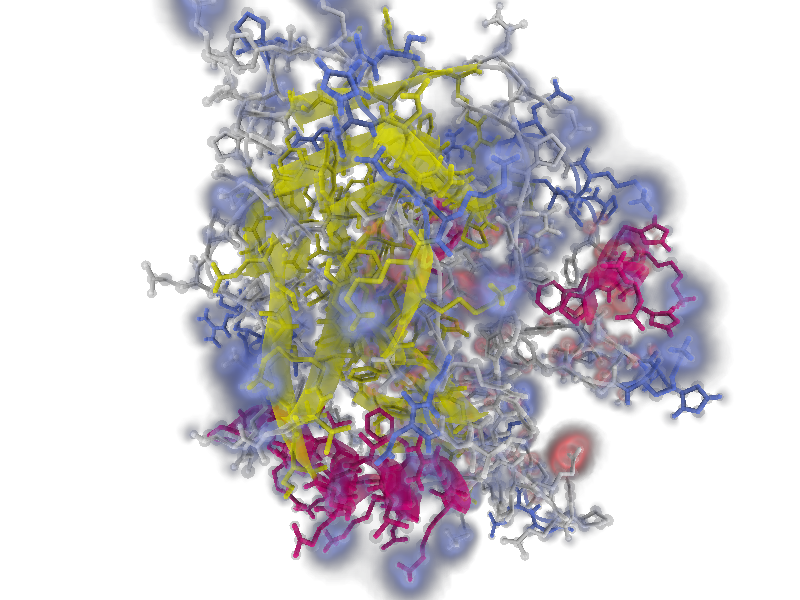
\includegraphics[height=1.2cm]{snapshots/performance/benchimage_Molecule}}} \\
    & \small VOL        & \small $71\times71\times71$ & \\
    & \small GEO        & \small 868k triangles & \\ % sticks + atoms (454182 + 407040 = 868k)
    & \small GEO        & \small 36k triangles & \\
    % & \multicolumn{3}{r}{\small \stencil: 64-32-16-8, \dloop: 8} \\
    \midrule
    
    Space       & \small VOL        & \small $256 \times 256 \times 256$ & 
    \multirow{5}{*}{\fbox{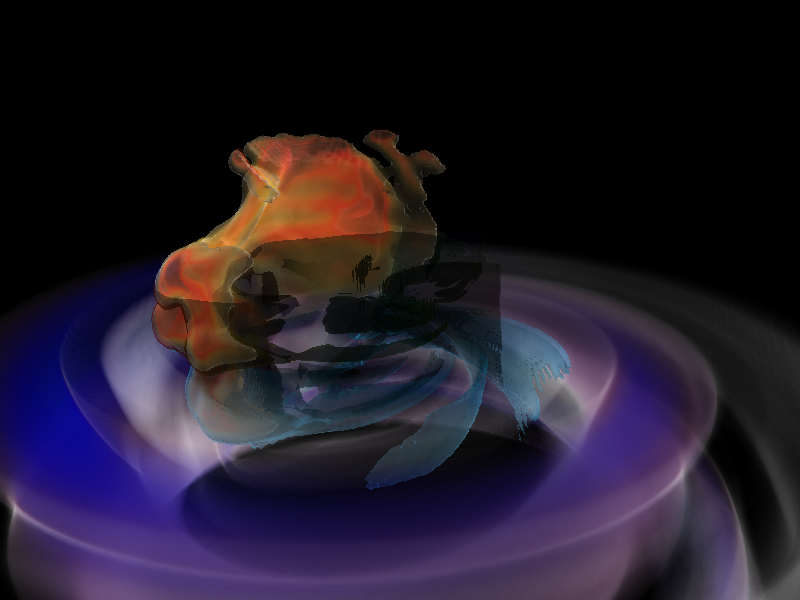
\includegraphics[height=1.2cm]{snapshots/performance/benchimage_Space}}} \\
    & \small VOL      & \small $256 \times 256 \times 256$ & \\
    & \small GEO        & \small 162k triangles & \\
    & \small GEO        & \small 100k triangles & \\
    & \small GEO        & \small 67k triangles & \\
    \midrule
    
    Neuro       & \small VOL        & \small $415\times487\times176$ & 
    \multirow{4}{*}{\fbox{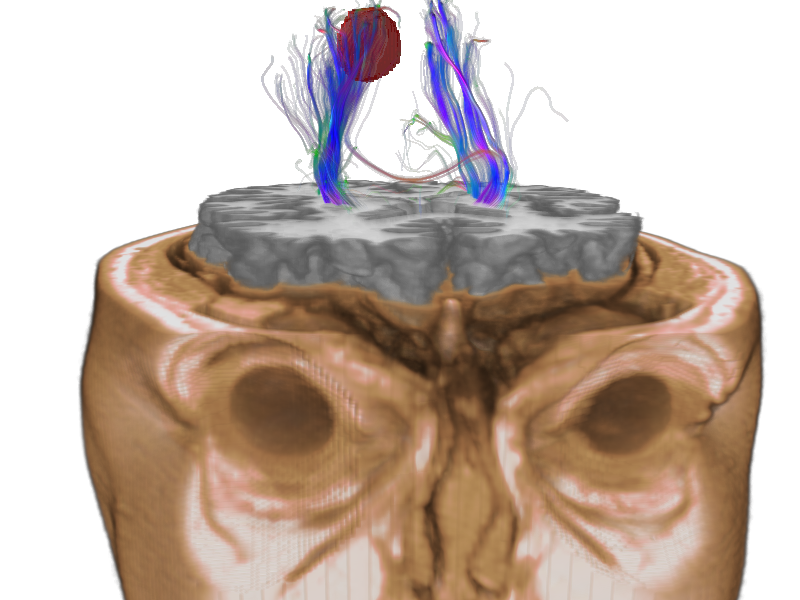
\includegraphics[height=1.2cm]{snapshots/performance/benchimage_Neuro}}} \\
    & \small VOL        & \small $367\times395\times150$ & \\
    & \small GEO        & 363k triangles & \\ % tumor (1088617 / 3 = 363k)
    & \small GEO        & \small $1678$ fibers & \\
    \midrule

    % 1184 1023 1037 1082 1089 879 1253 = 7547
    Flow        & \small VOL        & \small $76\times49\times45$ & 
    \multirow{4}{*}{\fbox{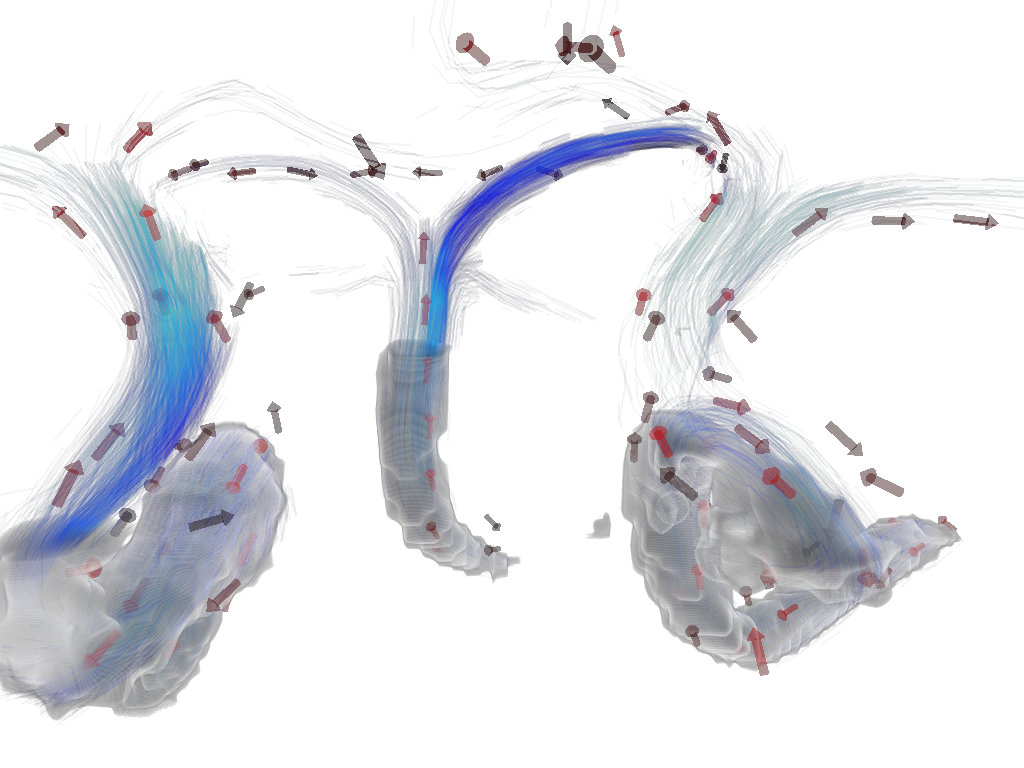
\includegraphics[height=1.2cm]{snapshots/performance/benchimage_Flow}}} \\
    & \small GEO        & \small $7.5$k streamlines & \\ % 7 x FiberRenderer (~1k each)
    & \small GEO        & \small $\approx100$ arrows & \\
    &  &  & \\
    \bottomrule
  \end{tabular}
\end{table}


%\todo{Reviewer 5: 
%  \begin{itemize}
%  \item Why the need for reporting test in two GPUs with the same architecture? 
%    And, still, only presenting results for one of them?
%  \item I would like to see comparisons with algorithms other than PPLL (e.g. FFB, DFB).
%  \end{itemize}
%}

%The full algorithm and its two proposed optimizations, the \stencil\ and the \dloop, were tested on four different GPUs. 
We have investigated how our optimizations improve the performance for each of the three algorithms for global memory management---FFB, DFB, and PPLL---presented in Section~\ref{sec:oit-global}. %%Section~\ref{sec:ab-merged}. 
For each choice of algorithm for global management we have measured the performance of four configurations for local memory management; no optimizations (static buffers), \stencil{}, \dloop{}, and \stencil{}+\dloop{}. 
For \stencil{}, depth segments were chosen as powers of two, starting at $32$ (Space), $64$ (Neuro), and $128$ (Neuro, Flow). 
Trying to allocate a \bArray{} to hold all depth layers of the Neuro scene resulted in driver crashes, thus only the first $128$ layers were resolved for the `base' and \stencil{} configurations (\dloop{} is capable of resolving higher complexities with smaller \bArray{}s). 
All performance for \dloop{} were timed with a \bArray{} of size $8$. 
Benchmark results are depicted in Figure~\ref{fig:performance} organized by scenes (rows), global algorithms (major columns), and GPUs (minor columns). 
Scene configurations can be found in Table~\ref{tab:data} including details on data sources. 
For each test, frame times were computed as the average over $30$s of rendering as the camera was rotated around the object at fixed distance, starting at the initial frame depicted in the table. 
Early ray termination was active with an alpha limit of $0.98$ for all benchmarks except the synthetic case in Figure~\ref{fig:viewdep-quad}. 

Due to an unforeseen performance penalty, we were unable to achieve results for the DFB on the same level as reported in~\cite{Maule2012}. 
The penalty manifested as a $50\,$ms--$200\,$ms delay associated with the context switch between CUDA/Thrust and OpenGL required by the `scan' step as described by Maule~\etal{}~\cite{Maule2012}. 
The penalty is persistent across GPUs and drivers and was present also in a minimal stand-alone DFB implementation. \todo{rewrite!/M}
The results for the DFB approach shown in Figure~\ref{fig:performance} include this penalty.

Evidenced by the performance graphs, both \stencil{} and \dloop{} are capable of providing significant performance gains for a large variety of configurations. 
The average gains for \stencil{} and \dloop{} are $3$ and $8$ times respectively when averaged over scenes and GPUs. %perfnumber
For highly complex or more homogeneous scenes, the improvement gained through \stencil{} drops off as the expensive pixels become a bottle neck. 
\dloop{} maintains a significant speedup even in these scenarios, particularly when early-ray-termination is activated. 
Additionally, we also measured a synthetic worst-case scenario (Figure~\ref{fig:viewdep-quad}) where the number of complex pixels approaches $100\%$ screen coverage. 
The results confirm that performance for \stencil{} (as expected) approaches that of statically implemented buffers while \dloop{} maintains a $3.6$ times speed increase. 



\begin{figure}[t]
  \centering
  \begin{minipage}{1.0\linewidth}\centering 
    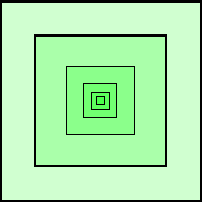
\includegraphics[width=0.14\linewidth]{figures/quads1}\hfill 
    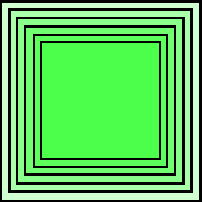
\includegraphics[width=0.14\linewidth]{figures/quads2}\hfill 
    
\includegraphics[width=0.14\linewidth]{figures/quads3}\hfill 
    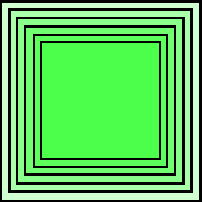
\includegraphics[width=0.14\linewidth]{figures/quads2}\hfill 
    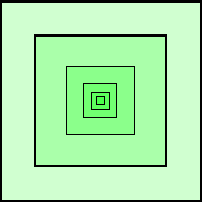
\includegraphics[width=0.14\linewidth]{figures/quads1}\hfill \hspace{6mm}
  \end{minipage}
  % 
  \begin{minipage}{1.0\linewidth}\centering
    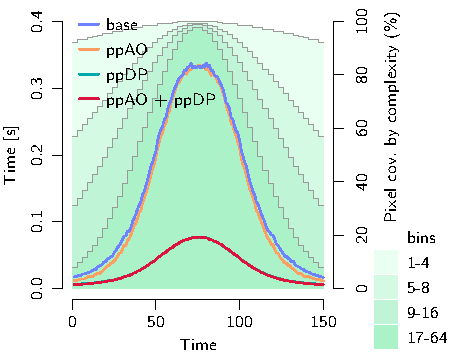
\includegraphics[width=\linewidth]{figures/plot-viewdep-quad-tall} 
  \end{minipage}
  \caption{\label{fig:viewdep-quad}%
    Performance and complexity graphs as a function of time for a synthetic test scene. 
    The scene consists of 64 quads orthogonal to the viewing direction (order randomized in depth). 
    The middle of the plot corresponds to a worst-case scenario where nearly all pixels have near maximum depth complexity. 
    Rendering times (left y-axis) are shown as line plots and \dch{}s as bar charts of pixel coverage (right y-axis). 
  }
\end{figure}


\section{Conclusions and Future Work}
\label{sec:conclusion}

%\todo{Reviewer 5: 
%  \begin{itemize}
%  \item You claim to have presented a visualization technique, but what I saw was an increment over a known OIT rendering technique (PPLL).
%  \item Your conclusion is not a conclusion; it only sums up all that you already said before.
%  \end{itemize}
%}
%
%\begin{itemize}
%\item dependent on application case
%  \begin{itemize}
%  \item volume gives context (flow, space)
%  \item geometry gives context (protein)
%  \item relation between different geometries (medical data, protein?)
%  \end{itemize}
%\end{itemize}

In this paper, we have introduced a high performance rendering algorithm which supports the interactive exploration of complex hybrid data. 
Two adaptive data handling schemes were developed based on the observations made when analyzing the depth complexity (using \dch{}s) of hybrid data sets as acquired in modern imaging-based sciences. 
%By minimizing the allocated local cache memory (\stencil) and performing a delayed depth sorting (\dloop), we are able to improve the previously inefficient management of local GPU caches caused by a few pixel with prohibitively high depth complexities. 
%The two optimizations were explicitly designed to better adapt the rendering algorithm to the rapidly decreasing \dch{}s commonly found in hybrid data scenes. 
Of the two, \dloop{} is better equipped to deal with very high complexities but does so at the cost of potential artifacts from z-fighting while \stencil{} performs well for moderate complexities with exact results. 
Both methods can also be combined to achieve support for high depth complexities while guaranteeing a minimum number of correctly blended samples. 

Our work enables fusion of volumetric data with semi-transparent geometry for scenes that could not be rendered at interactive frame rates with previous approaches. 
We believe the developed algorithms could be applicable also to other areas of visualization that utilize \ab{} techniques and that their applicability should be further strengthened since both \stencil{} and \dloop{} are compatible with most leading \ab{} solution for global memory management. 
%We have shown the performance gain achieved by our method and discussed its application to real-world data sets. 

In the future, we see several opportunities to improve the proposed method. 
For instance, by combining our algorithm with space partitioning data structures, we might even get higher performance gains. 
However, perhaps an even more interesting avenue would be to analyze the trade-offs that can be made when blending multiple semi-transparent layers. 
Apart from this, the proposed technique also paves the way for new visualization techniques. 
For instance, it will now be possible to encode fiber tracking uncertainty in the alpha channel of the visualized fibers, without eliminating the possibility to also visualize a co-registered volume. 

%%% if specified like this the section will be ommitted in review mode
\section{Acknowledgments}
\label{sec:acknowledgments}

\todo{insert acknowledgments here!}
The authors wish to thank A, B, C. This work was supported in part by
a grant from XYZ.\\
%
% GRANTS
% Cyril Crassin
% Maule et al.
% Data providers
%

\begin{figure*}[p]
  \centering
  %% 
  %% create final image first to ensure that it is labeled with (a)
  %% do not show it but store it in a box for later use    
  \savebox\savedProteinBox{%
    \begin{minipage}[b]{0.51\linewidth}%
      \centering%
      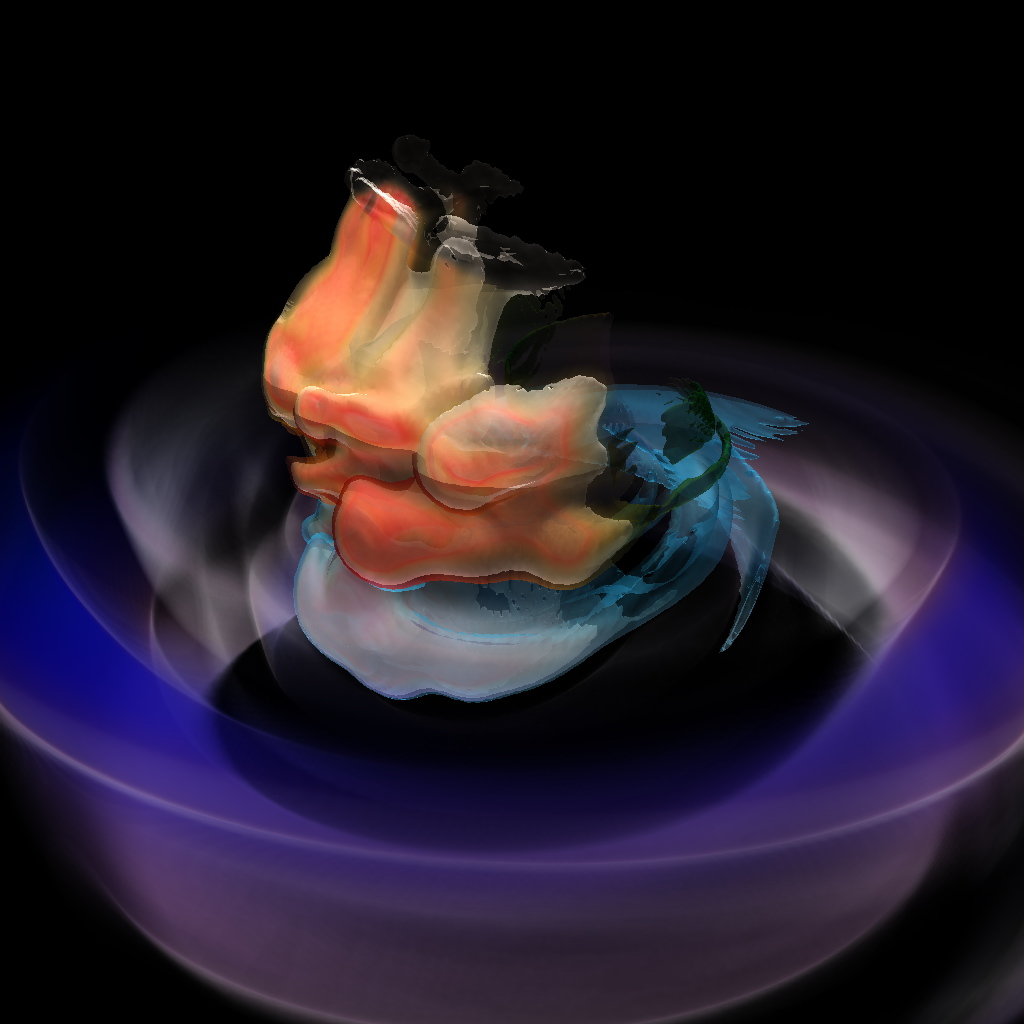
\includegraphics[width=\linewidth]{snapshots/space/space}%
      \subcaption{\label{fig:sub:space}%
        hybrid visualization
      }%
    \end{minipage}%
  }
  \settoheight{\boxheight}{\usebox\savedProteinBox}
  % 
  \begin{minipage}[b][\boxheight][b]{0.24\linewidth}
    \centering%
    \begin{minipage}[t]{0.98\linewidth}
      \centering
      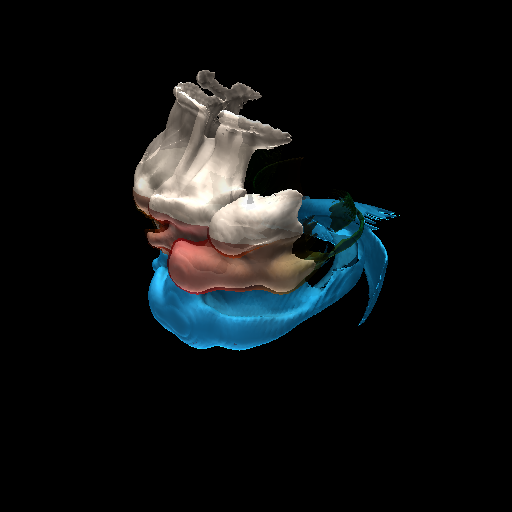
\includegraphics[width=\textwidth]{snapshots/space/space-only-isos}
      \subcaption{\label{fig:sub:space-geom}%
        geometric data
      }
    \end{minipage}%
    \vfill%
    \begin{minipage}[b]{0.98\linewidth}
      \centering
      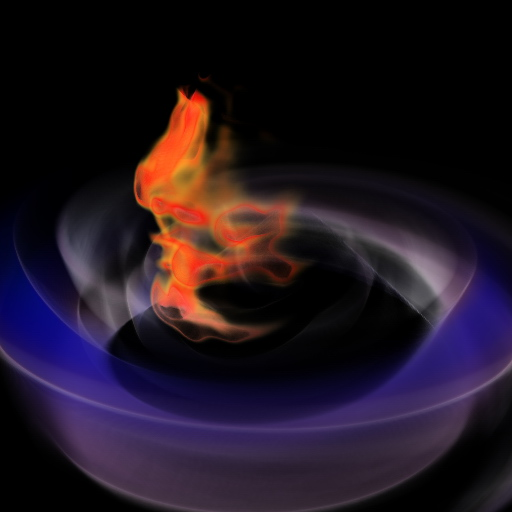
\includegraphics[width=\textwidth]{snapshots/space/space-only-vols}
      \subcaption{\label{fig:sub:space-vols}%
        volume data
      }
    \end{minipage}%
  \end{minipage}%
  \hfill%
  %% central image
  \usebox\savedProteinBox
  \hfill%
  \begin{minipage}[b][\boxheight][b]{0.24\linewidth}
    \centering%
    \begin{minipage}[t]{0.98\linewidth}
      \centering
      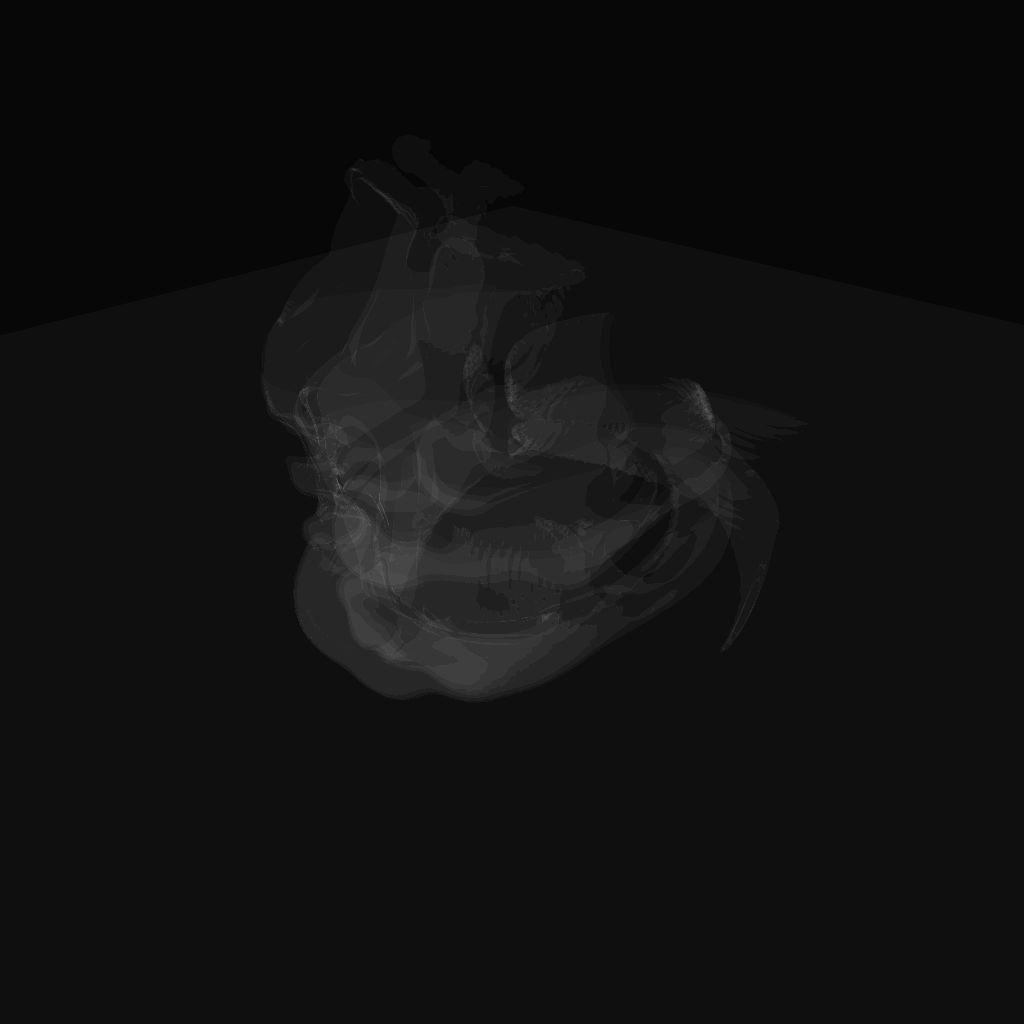
\includegraphics[width=\linewidth]{snapshots/space/space_dci-wp64}%
      \subcaption{\label{fig:sub:space-dci}%
        depth complexity
      }
    \end{minipage}%
    \vfill%
    \begin{minipage}[b]{0.98\linewidth}
      \centering
      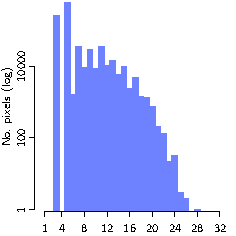
\includegraphics[width=1\linewidth]{figures/plot-dch-space}\vspace{-2mm}
      \subcaption{\label{fig:sub:space-dch}%
        depth complexity histogram
      }
    \end{minipage}%
  \end{minipage}%
  % 
  \caption{\label{fig:space}%
    Visualization of a solar mass ejection simulation data used for predicting space weather. 
    (\subref{fig:sub:space}) final rendering of hybrid visualization.
    (\subref{fig:sub:space-geom}) three geometric representations.
    (\subref*{fig:sub:space-vols}) volumetric data sources. %% depicting inner and outer extents of the simulation at different resolution.
    (\subref{fig:sub:space-dci}) image-space depth complexity (re-scaled for representational purposes). 
    (\subref{fig:sub:space-dch}) depth complexity histogram (DCH, log scale).
    Our improved \ab{} algorithm achieves up to four times \todo{check!} the performance compared to existing approaches.
  }
\end{figure*}

\begin{figure*}[p]
  \centering
  \begin{minipage}[b]{0.26\linewidth}\centering
    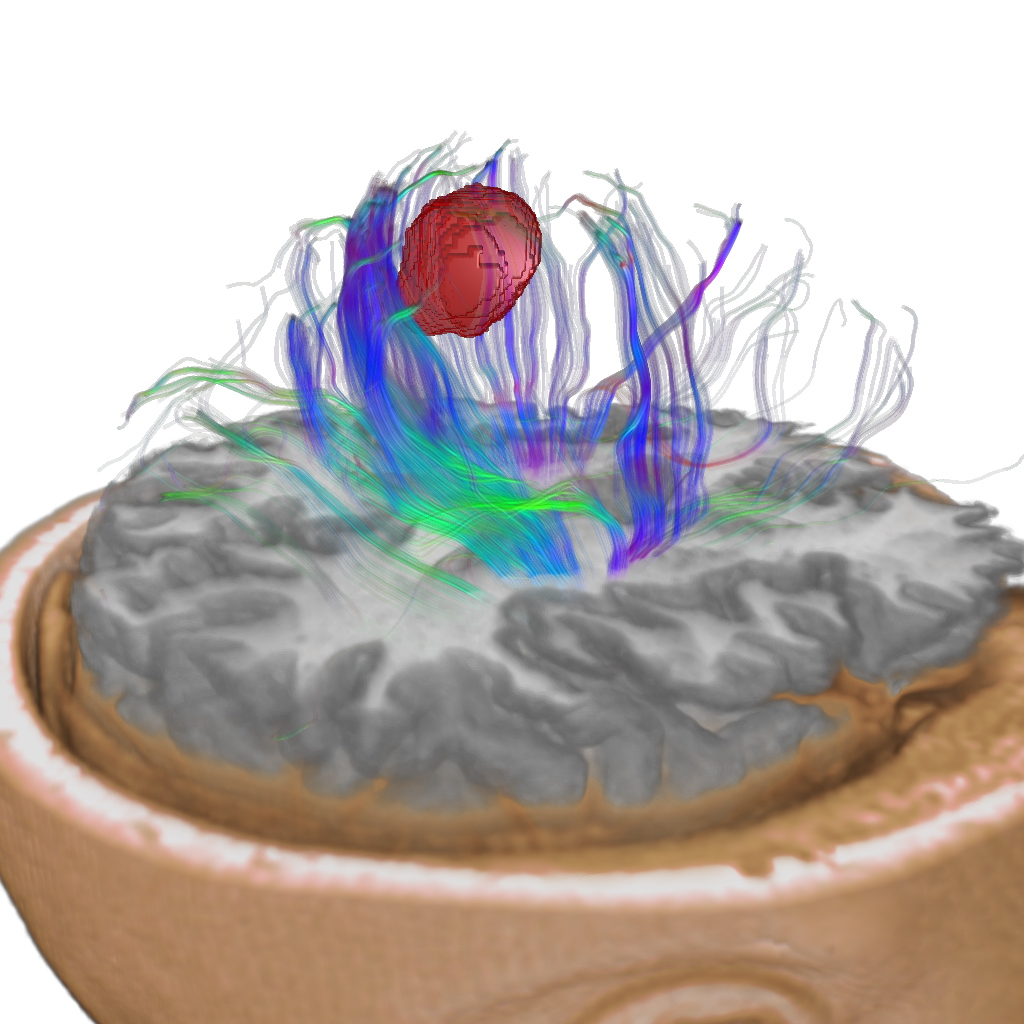
\includegraphics[width=0.98\linewidth]{snapshots/dti/cgf/screenshot_Neuro}%
    \subcaption{\label{fig:sub:neuro}%
      neurosurgical planning
    }
  \end{minipage}\hfill
  \begin{minipage}[b]{0.22\linewidth}\centering
    % 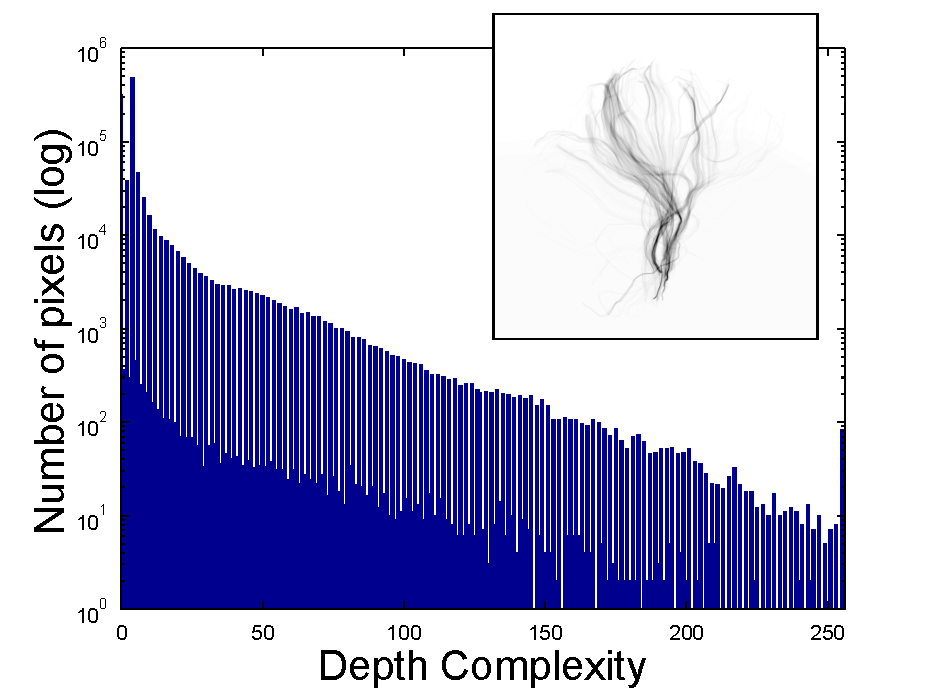
\includegraphics[width=0.98\linewidth]{snapshots/dti/cgf/dci-dch_Neuro_dch-256-max255}
    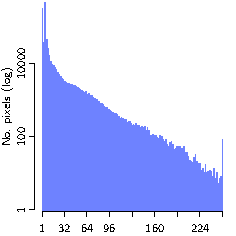
\includegraphics{figures/plot-dch-neuro}
    \subcaption{\label{fig:sub:neuro-dch}%
      depth complexity
    }
  \end{minipage}\hfill
  \begin{minipage}[b]{0.26\linewidth}\centering
    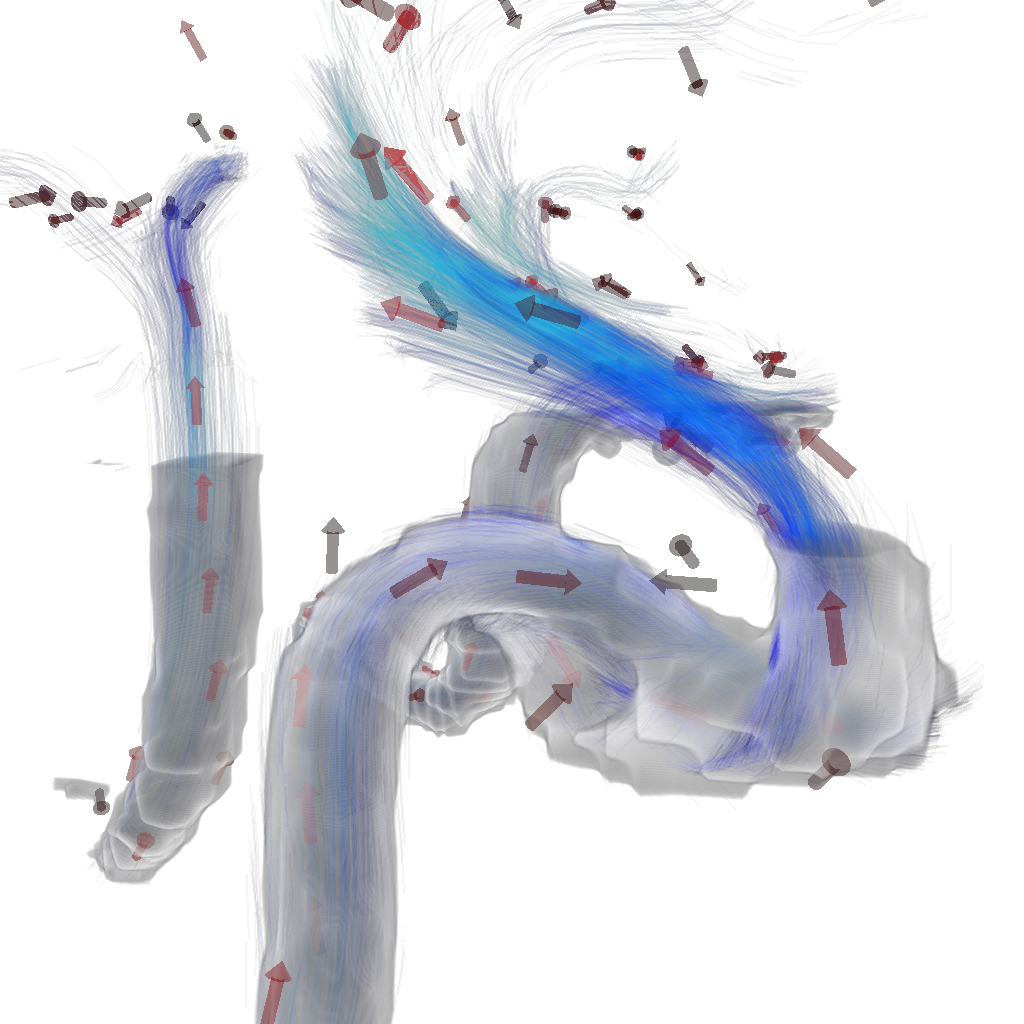
\includegraphics[width=0.98\linewidth]{snapshots/flow/cgf/screenshot_Flow}
    \subcaption{\label{fig:sub:flow}%
      blood flow
    }
  \end{minipage}\hfill
  \begin{minipage}[b]{0.22\linewidth}\centering
    % \includegraphics[width=0.98\linewidth]{snapshots/flow/cgf/dci-dch_Flow_dch-128-max79}
    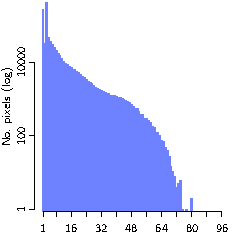
\includegraphics{figures/plot-dch-flow}
    \subcaption{\label{fig:sub:flow-dch}%
      depth complexity
    }
  \end{minipage}
  % 
  \caption{\label{fig:neuro-flow}%
    Fused visualization of hybrid data is becoming an important tool in a variety of fields. 
    (\subref{fig:sub:neuro}) visualization used for neurosurgical planning.
    (\subref{fig:sub:flow}) visualization used to asses the blood flow in the carotid artery. 
    Both scenes contain multiple sources of semi-transparent geometry as well as volumetric data. 
    %% Performing these rendering in real time is essential in order for a user to explore the data, but challenging due to the high depth complexities of the scenes. 
    (\subref{fig:sub:neuro-dch}) and (\subref{fig:sub:flow-dch}) depict the rapidly decreasing depth complexity histograms (\dch{}s, log scale). %perfnumber
    %% with maximum depth complexities of $294$ (neuro) and $79$ (flow), respectively. 
  }
\end{figure*}


%\begin{table*}[t]
%\centering
%		\begin{tabular}{| p{1.1cm} || c | c || c | c | c || c || c | c || c | c || c |}
%		\hline 
%			& & & \multicolumn{7}{c|}{Performance Configurations (timings in FPS)} & \\
%			& & & \multicolumn{3}{c||}{PPLL}    &    \multicolumn{1}{c||}{PPLL}    &    \multicolumn{2}{c||}{PPLL}    &    \multicolumn{1}{c|}{PPLL} & \\
%			& & & \multicolumn{3}{c||}{~}    &    \multicolumn{1}{c||}{+ppAO}    &    \multicolumn{2}{c||}{+ppDP}    &    \multicolumn{1}{c|}{+ppAO} & \\
%			& & & \multicolumn{3}{c||}{~}    &    \multicolumn{1}{c||}{~}    &    \multicolumn{2}{c||}{~}    &    \multicolumn{1}{c|}{+ppDP} & \\
%		
%		Setup 			& Data & Data size  & 32   & 64    & 128  & 128---8  & 8*    & 16*   & 8*,8 & \% \\
%		\hline\hline
%			
%		Protein     & \small VOL        & \small $127\times127\times127$ & 53.08 & 25.34 & 10.30 & 66.71 & 87.03 & 74.68 & 92.85 & \textbf{3.6X} \\
%		        	  & \small VOL        & \small $71\times71\times71$ & (NC) &   		&  			&      &       &     	&     &  \\
%		            %& \small VOL        & \small $71\times71\times71$ &   	  &       &  	    &       &       &  	    &     &  \\
%		            & \small GEO        & \small 45k triangles &   	  &       &  	    &       &       &  	    &     &  \\
%		            & \small GEO        & \small 36k triangles &   	  &       &  	    &       &       &  	    &    &   \\
%		\hline
%		
%		Space       & \small VOL        & \small $256 \times 256 \times 256$ & 9.86 & 4.21 & 3.22 & 28.56 & 34.86 & 24.80 & 36.15 &  \textbf{8.5X} \\
%		Weather  & \small VOL      & \small $256 \times 256 \times 256$ & (NC) &       &      	&       &       &     	& & \\
%		            & \small GEO        & \small 162k triangles              &   	  &       &  	    &       &       &  	    & & \\
%		            & \small GEO        & \small 100k triangles              &   	  &       &  	    &       &       &  	    & & \\
%		            & \small GEO        & \small 67k triangles               &   	  &       &  	    &       &       &  	    & & \\
%		\hline
%		
%		Neuro       & \small VOL        & \small $415\times487\times176$ & 21.19 & 9.25 & 3.29 & 7.94 & 39.37 & 32.04 & 40.73 & --- \\
%		        	  & \small VOL        & \small $367\times395\times150$ & (NC) & (NC)  & (NC) & (NC)&       &  	   &       & \\
%		            & \small GEO        & \small $54\times52\times29$    &   	  &      &  	  &      &       &  	   &       & \\
%		            & \small GEO        & \small $1678$ streamlines           &    	&      &  	  &      &       &  	   &       & \\
%		\hline
%		
%		Flow        & \small VOL        & \small $76\times49\times45$ & 19.25 & 9.35 & 3.93 & 29.43 & 32.95 & 27.05 & 34.31 &  \textbf{3.6X} \\
%			  & \small GEO        & \small $1986$ streamlines     & (NC)  &      &  	  &      &       &  	   &      &  \\
%		            & \small GEO        & \small $\approx100$ arrows             &   	  &      &  	  &      &       &  	   &       & \\
%		\hline
%	  \end{tabular}
%	\caption{%
%	Performance measurements of our algorithm. 
%	The numerical labels (top) depicts the size of the \bArray. 
%	A * indicates the array size used for looping (\dloop). 
%	The (NC = Not correct) label indicates that the configuration was unable to render all fragments for one or more pixels due to overflow in the local array. 
%	For the Neuro scene, no configuration that relied on single usage of static arrays were capable of rendering the image without discarding unresolved samples. 
%          \todo{Reviewer 5: 
%            what is the maximum depth complexity for each scene? 
%            i.e.\ does not make sense to present results for a local array size of 128 for a scene with max.\ depth complexity of 64 (it is misleading). 
%            What do the ``*'' mean? What is the ``\%'' column?
%          }
%        }
%	\label{tab:performance}
%\end{table*}


%\bibliographystyle{eg-alpha}
\bibliographystyle{eg-alpha-doi}

\bibliography{literature}

\end{document}




